%%%%%%%%%%%%%%%%%%%%%%%%%%%%%%%%%%%%%%%%%%%%%%%%%%%%%%%%%%%%%%%%%
%%%%%%%%%%%%%%%%%%%%%%%%%%%%%%%%%%%%%%%%%%%%%%%%%%%%%%%%%%%%%%%%%
\chapter{Basic and complex PK Macros}
\label{sec:PKMacrosAppendix}

%%%%%%%%%%%%%%%%%%%%%%%%%%%%%%%%%%%%%%%%%%%%%%%%%%%%%%%%%%%%%%%%%%%%%%
\section{PREDPP 1-4/10-12 models}

%%%%%%%%%%%%%%%%%%%%%%%%%%%%%%%%%%%%%%%%%%%%%%%%%%%%%%%%%%%%%%%%%%%%%%
\subsection{ADVAN1, TRANS1 -- 1-comp IV input}
\label{subsubsec:ADVAN1}
ODE formulation:
\begin{align}
\frac{dAc}{dt} &= - k \times Ac  \nonumber
\end{align}


\begin{figure}[htbp!]
\centering
 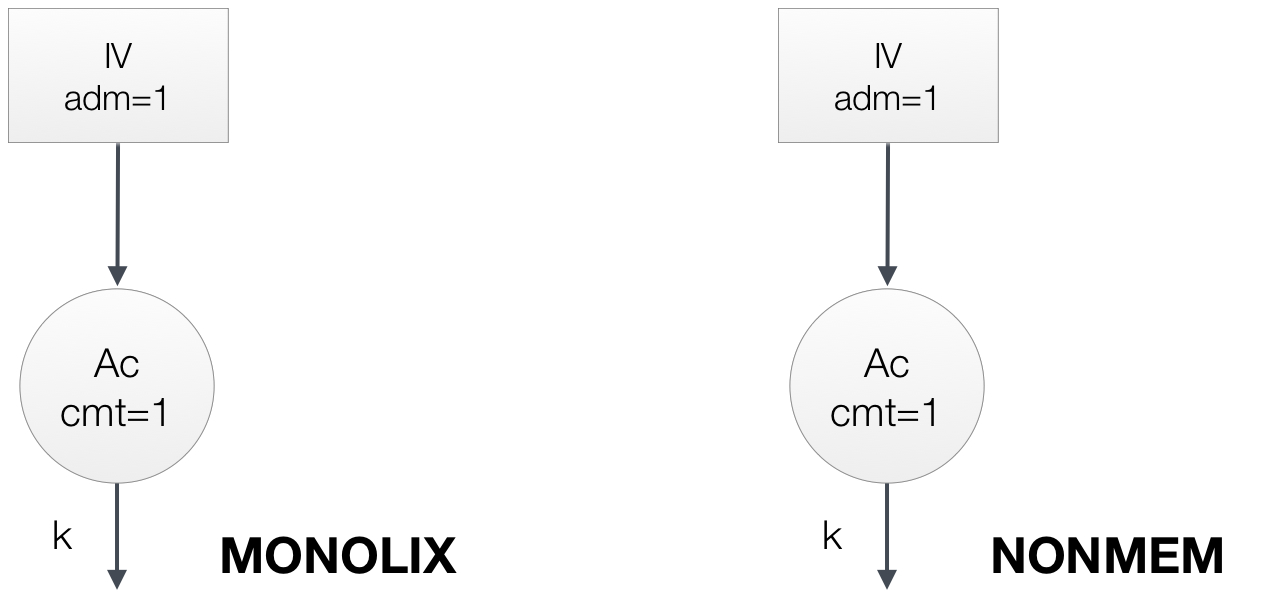
\includegraphics[width=100mm]{pics/Advan1}
\caption{ADVAN1 model, in this case compartment numbering is identical.}
\label{fig:Advan1}
\end{figure}

\begin{table}[ht!]
\footnotesize
\parbox{.5\linewidth}{
\centering
\begin{tabular}{ccccc}
  \hline
   \multicolumn{5}{c}{\textbf{MONOLIX}} \\
  \hline
ID & TIME & AMT & \textbf{ADM} & Y  \\
  \hline
1  & 0        & 10   & \textbf{1} & .       \\
1  & 2        & .      & .   & 5      \\
... &  ...      &  ...   &  ...   & ...  \\
\end{tabular}
}
\hfill
\parbox{.5\linewidth}{
\centering
\begin{tabular}{ccccc}
  \hline
   \multicolumn{5}{c}{\textbf{NONMEM}} \\
  \hline
ID & TIME & AMT & \textbf{\textcolor{red}{CMT}} & DV \\
  \hline
1  & 0        & 10   & \textbf{\textcolor{red}{1}}   & .    \\
1  & 2        & .      & 1    & 5   \\
... &  ...      &  ...   &  ... & ...  \\
\end{tabular}
}
\caption{MONOLIX and NONMEM datasets for the ADVAN1 model.}
\end{table}


\begin{table}[h!]
\setlength{\tabcolsep}{15pt}
\begin{center}
\begin{tabular}{l}
  \hline \hline
PK macro \\[-.25ex]
  \hline
\lstset{language=NONMEMdataSet}
\begin{lstlisting}
input = {V, k}
PK:
compartment(cmt=1, amount=Ac, volume=V)
iv(adm=1, cmt=1)
elimination(cmt=1, k)
\end{lstlisting}
%&
%\lstset{language=NONMEMdataSet}
%\begin{lstlisting}
%input = {V, k}
%PK:
%compartment(cmt=1, amount=Ac, volume=V)
%iv(adm=1, cmt=1)
%elimination(cmt=1, k)
%\end{lstlisting} 
\\
  \hline
\end{tabular}
\caption{PK macros  for the ADVAN1 model, as shown in Figure \ref{fig:ComplexModel1a} (left).}
\label{tab:advan1Table}
\end{center}
\end{table}


PharmML code\footnote{Only the ADVAN1 code example contains the parameter model, \xatt{pm1}, in which
all model parameters has to be defined. It is omitted in the remaining cases for simplicity.}
% The same holds for the \xelem{StructuralModel} tags}:
\lstset{language=XML}
\begin{lstlisting}
        <ParameterModel blkId="pm1">
            <!-- no IIV assumed for simplicity -->
            <SimpleParameter symbId="k"/>
            <SimpleParameter symbId="V"/>
        </ParameterModel>

        <StructuralModel blkId="sm1">
            <ct:Variable symbolType="real" symbId="Ac"/>
            
            <PKmacros>
                <Compartment>
                    <Value argument="cmt">
                        <ct:Int>1</ct:Int>
                    </Value>
                    <Value argument="amount">
                        <ct:SymbRef symbIdRef="Ac"/>
                    </Value>
                    <Value argument="volume">
                        <ct:SymbRef blkIdRef="pm1" symbIdRef="V"/>
                    </Value>
                </Compartment>
                
                <IV>
                    <Value argument="adm">
                        <ct:Int>1</ct:Int>
                    </Value>
                    <Value argument="cmt">
                        <ct:Int>1</ct:Int>
                    </Value>
                </IV>
                
                <Elimination>
                    <Value argument="cmt">
                        <ct:Int>1</ct:Int>
                    </Value>
                    <Value>
                        <ct:SymbRef blkIdRef="pm1" symbIdRef="k"/>
                    </Value>
                </Elimination>
            </PKmacros>
        </StructuralModel>
 \end{lstlisting}


%\cleardoublepage
%%%%%%%%%%%%%%%%%%%%%%%%%%%%%%%%%%%%%%%%%%%%%%%%%%%%%%%%%%%%%%%%%%%%%%
\subsection{ADVAN2, TRANS1 -- 1-comp 1st order input}
\label{subsubsec:advan2}
ODE formulation:
\begin{align}
\frac{dAd}{dt} &= -ka \times Ad \nonumber \\
\frac{dAc}{dt} &= ka \times Ad - k \times Ac  \nonumber
\end{align}


\begin{figure}[htbp!]
\centering
 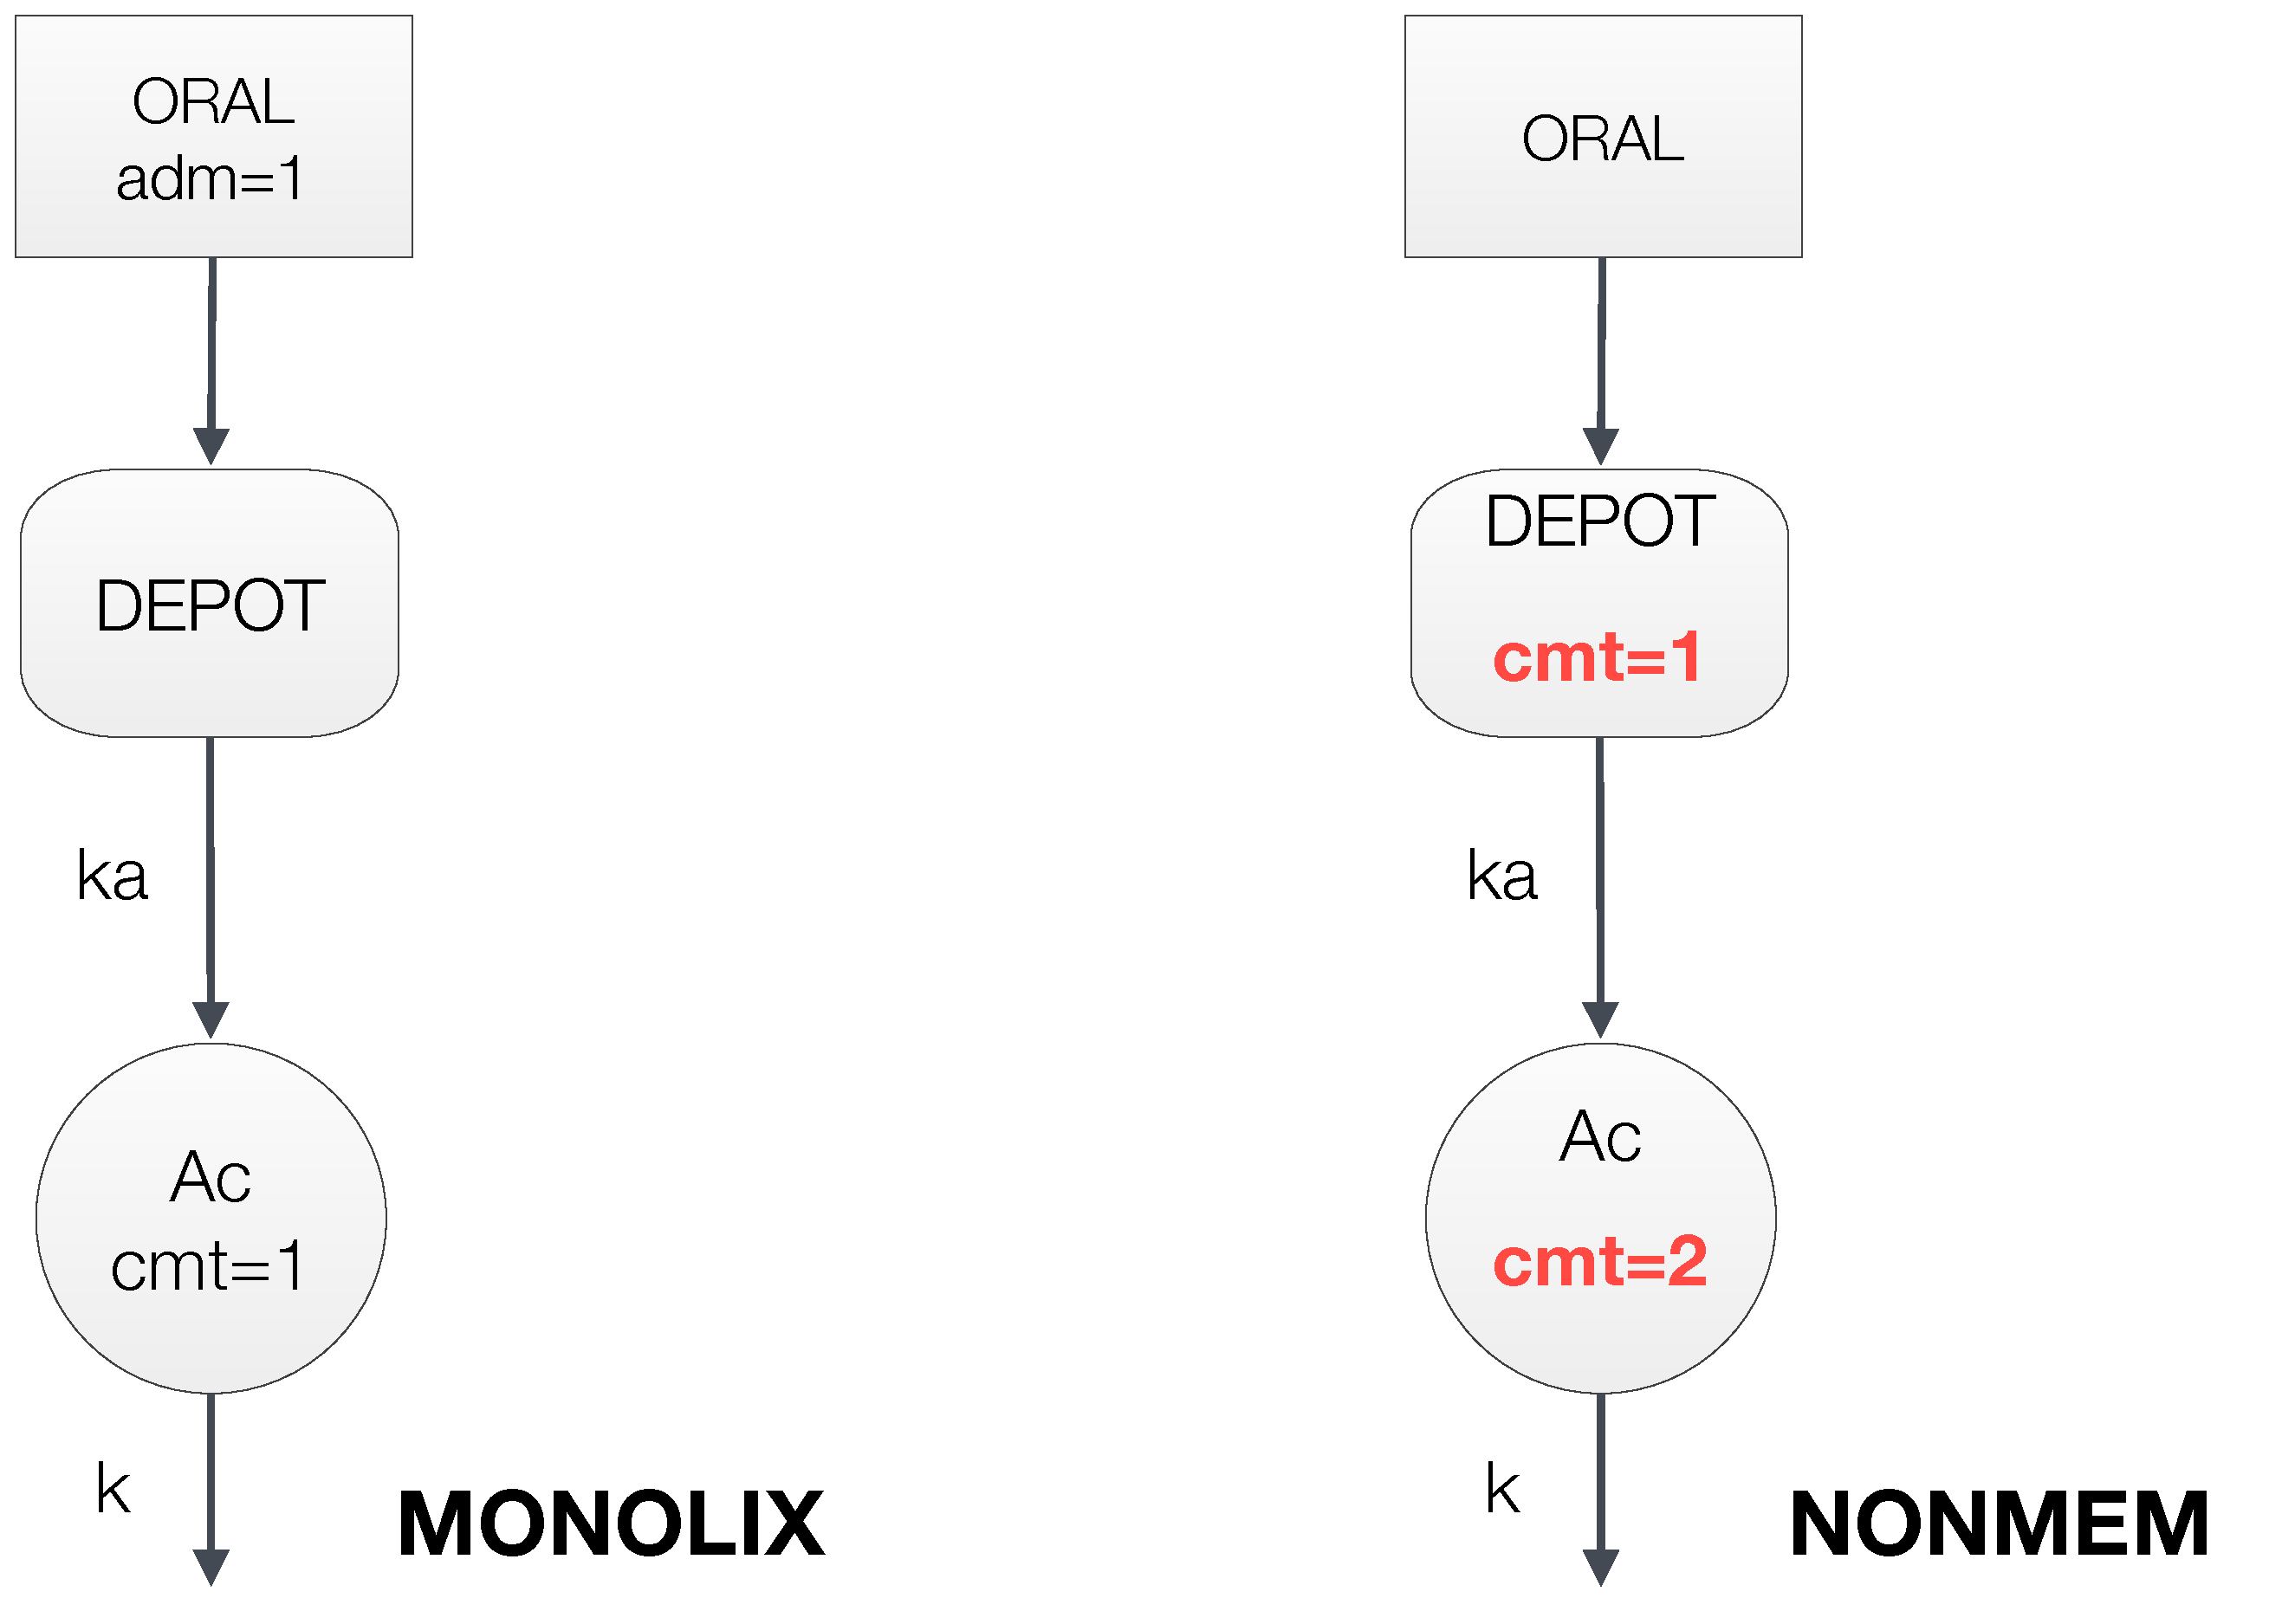
\includegraphics[width=100mm]{pics/Advan2}
\caption{ADVAN2 model, with compartment numbering dependent on the target tool.}
\label{fig:Advan2}
\end{figure}


\begin{table}[ht!]
\footnotesize
\parbox{.5\linewidth}{
\centering
\begin{tabular}{ccccc}
  \hline
   \multicolumn{5}{c}{\textbf{MONOLIX}} \\
  \hline
ID & TIME & AMT & \textbf{ADM} & Y \\
  \hline
1  & 0        & 10   & \textbf{1} & .       \\
1  & 2        & .      & .     & 5      \\
... &  ...      &  ...   &  ...  & ...   \\
\end{tabular}
}
\hfill
\parbox{.5\linewidth}{
\centering
\begin{tabular}{ccccc}
  \hline
   \multicolumn{5}{c}{\textbf{NONMEM}} \\
  \hline
ID & TIME & AMT & \textbf{\textcolor{red}{CMT}} & DV \\
  \hline
1  & 0        & 10   & \textbf{\textcolor{red}{1}}   & .    \\
1  & 2        & .      & 2    & 5   \\
... &  ...      &  ...   &  ... & ...  \\
\end{tabular}
}
\caption{MONOLIX and NONMEM datasets for the ADVAN2 model.}
\end{table}

\lstset{language=MLXTRANcode}
\begin{lstlisting}
\end{lstlisting}

\begin{table}[h!]
\setlength{\tabcolsep}{15pt}
\begin{center}
%\begin{tabular*}{.95\textwidth}{@{\extracolsep{\fill} } ll}
\begin{tabular}{l}
  \hline \hline
PK macro  \\[-.25ex]
  \hline
\lstset{language=NONMEMdataSet}
\begin{lstlisting}
input = {ka, V, k}
PK:
compartment(cmt=1, amount=Ac, volume=V)
oral(adm=1, cmt=1, ka)
elimination(cmt=1, k)
\end{lstlisting}
%&
%\lstset{language=NONMEMdataSet}
%\begin{lstlisting}
%input = {ka, V, k}
%PK:
%compartment(cmt=1, amount=Ac, volume=V)
%[*compartment(cmt=2, amount=Depot)*]
%oral(adm=1, [*fromCmt=2,*] cmt=1, ka)
%elimination(cmt=1, k)
%\end{lstlisting} 
\\
  \hline
\end{tabular}
\caption{PK macros  for the ADVAN2 model, as shown in Figure \ref{fig:Advan2} (left).}
\label{tab:advan2Table}
\end{center}
\end{table}

PharmML code:
\lstset{language=XML}
\begin{lstlisting}
        <StructuralModel blkId="sm2">
            <ct:Variable symbolType="real" symbId="Ac"/>
            
            <PKmacros>
                <Compartment>
                    <Value argument="cmt">
                        <ct:Int>1</ct:Int>
                    </Value>
                    <Value argument="amount">
                        <ct:SymbRef symbIdRef="Ac"/>
                    </Value>
                    <Value argument="volume">
                        <ct:SymbRef blkIdRef="pm1" symbIdRef="V"/>
                    </Value>
                </Compartment>
                
                <Oral>
                    <Value argument="adm">
                        <ct:Int>1</ct:Int>
                    </Value>
                    <Value argument="cmt">
                        <ct:Int>1</ct:Int>
                    </Value>
                    <Value>
                        <ct:SymbRef blkIdRef="pm1" symbIdRef="ka"/>
                    </Value>
                </Oral>
                
                <Elimination>
                    <Value argument="cmt">
                        <ct:Int>1</ct:Int>
                    </Value>
                    <Value>
                        <ct:SymbRef blkIdRef="pm1" symbIdRef="k"/>
                    </Value>
                </Elimination>
            </PKmacros>
        </StructuralModel>
\end{lstlisting}


%\cleardoublepage
%%%%%%%%%%%%%%%%%%%%%%%%%%%%%%%%%%%%%%%%%%%%%%%%%%%%%%%%%%%%%%%%%%%%%%
\subsection{ADVAN3, TRANS1 -- 2-comp IV input}
ODE formulation:
\begin{align}
\frac{dAc}{dt} &= -k_{12}\times Ac + k_{21} \times Ap - k \times Ac  \nonumber \\
\frac{dAp}{dt} &= k_{12}\times Ac - k_{21} \times Ap  \nonumber
\end{align}

\begin{figure}[htbp!]
\centering
 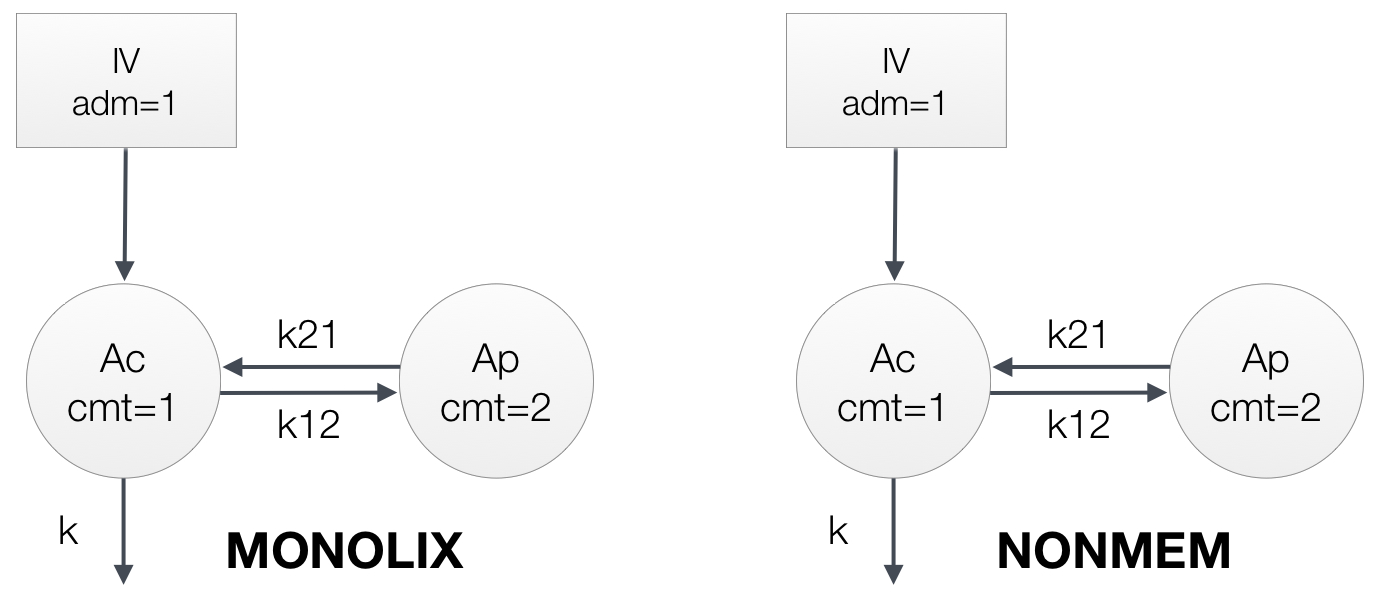
\includegraphics[width=110mm]{pics/Advan3}
\caption{ADVAN3 model, in this case compartment numbering is identical.}
\label{fig:Advan3}
\end{figure}


\begin{table}[ht!]
\footnotesize
\parbox{.5\linewidth}{
\centering
\begin{tabular}{ccccc}
  \hline
   \multicolumn{5}{c}{\textbf{MONOLIX}} \\
  \hline
ID & TIME & AMT & \textbf{ADM} & Y \\
  \hline
1  & 0        & 10   & \textbf{1} & .       \\
1  & 2        & .      & .    & 5    \\
... &  ...      &  ...   &  ... & ...    \\
\end{tabular}
}
\hfill
\parbox{.5\linewidth}{
\centering
\begin{tabular}{ccccc}
  \hline
   \multicolumn{5}{c}{\textbf{NONMEM}} \\
  \hline
ID & TIME & AMT & \textbf{CMT} & DV \\
  \hline
1  & 0        & 10   & \textbf{1}   & .    \\
1  & 2        & .      & 2    & 5   \\
... &  ...      &  ...   &  ... & ...  \\
\end{tabular}
}
\caption{MONOLIX and NONMEM datasets for the ADVAN3 model.}
\end{table}


\begin{table}[h!]
\setlength{\tabcolsep}{15pt}
\begin{center}
%\begin{tabular*}{.95\textwidth}{@{\extracolsep{\fill} } ll}
\begin{tabular}{l}
  \hline \hline
PK macro \\[-.25ex]
  \hline
\lstset{language=NONMEMdataSet}
\begin{lstlisting}
input = {V, k, k12, k21}
PK:
compartment(cmt=1, amount=Ac, volume=V)
peripheral(k12, k21, amount=Ap)
iv(adm=1, cmt=1)
elimination(cmt=1, k)
\end{lstlisting}
%&
%\lstset{language=NONMEMdataSet}
%\begin{lstlisting}
%input = {V, k, k12, k21}
%PK:
%compartment(cmt=1, amount=Ac, volume=V)
%peripheral(k12, k21, amount=Ap)
%iv(adm=1, cmt=1)
%elimination(cmt=1, k)
%\end{lstlisting} 
\\
  \hline
\end{tabular}
\caption{PK macros  for the ADVAN3 model, as shown in Figure \ref{fig:Advan3} (left).}
\label{tab:advan3Table}
\end{center}
\end{table}


PharmML code:
\lstset{language=XML}
\begin{lstlisting}
        <StructuralModel blkId="sm3">
            
            <ct:Variable symbolType="real" symbId="Ac"/>
            <ct:Variable symbolType="real" symbId="Ap"/>
            
            <PKmacros>
                <Compartment>
                    <Value argument="cmt">
                        <ct:Int>1</ct:Int>
                    </Value>
                    <Value argument="amount">
                        <ct:SymbRef symbIdRef="Ac"/>
                    </Value>
                    <Value argument="volume">
                        <ct:SymbRef symbIdRef="V"/>
                    </Value>
                </Compartment>
                
                <Peripheral>
                    <Value>
                        <ct:SymbRef symbIdRef="k12"/>
                    </Value>
                    <Value>
                        <ct:SymbRef symbIdRef="k21"/>
                    </Value>
                    <Value argument="amount">
                        <ct:SymbRef symbIdRef="Ap"/>
                    </Value>
                </Peripheral>
                
                <IV>
                    <Value argument="adm">
                        <ct:Int>1</ct:Int>
                    </Value>
                    <Value argument="cmt">
                        <ct:Int>1</ct:Int>
                    </Value>
                </IV>
                
                <Elimination>
                    <Value argument="cmt">
                        <ct:Int>1</ct:Int>
                    </Value>
                    <Value>
                        <ct:SymbRef symbIdRef="k"/>
                    </Value>
                </Elimination>
            </PKmacros>
        </StructuralModel>
\end{lstlisting}


%\cleardoublepage
%%%%%%%%%%%%%%%%%%%%%%%%%%%%%%%%%%%%%%%%%%%%%%%%%%%%%%%%%%%%%%%%%%%%%%
\subsection{ADVAN4, TRANS1 -- 2-comp 1st order input}
ODE formulation:
\begin{align}
\frac{dAd}{dt} &= -ka \times Ad \nonumber \\
\frac{dAc}{dt} &= ka \times Ad - k_{12} \times Ac + k_{21} \times Ap - k \times Ac  \nonumber \\
\frac{dAp}{dt} &= k_{12} \times Ac - k_{21} \times Ap  \nonumber
\end{align}

\begin{figure}[htbp!]
\centering
 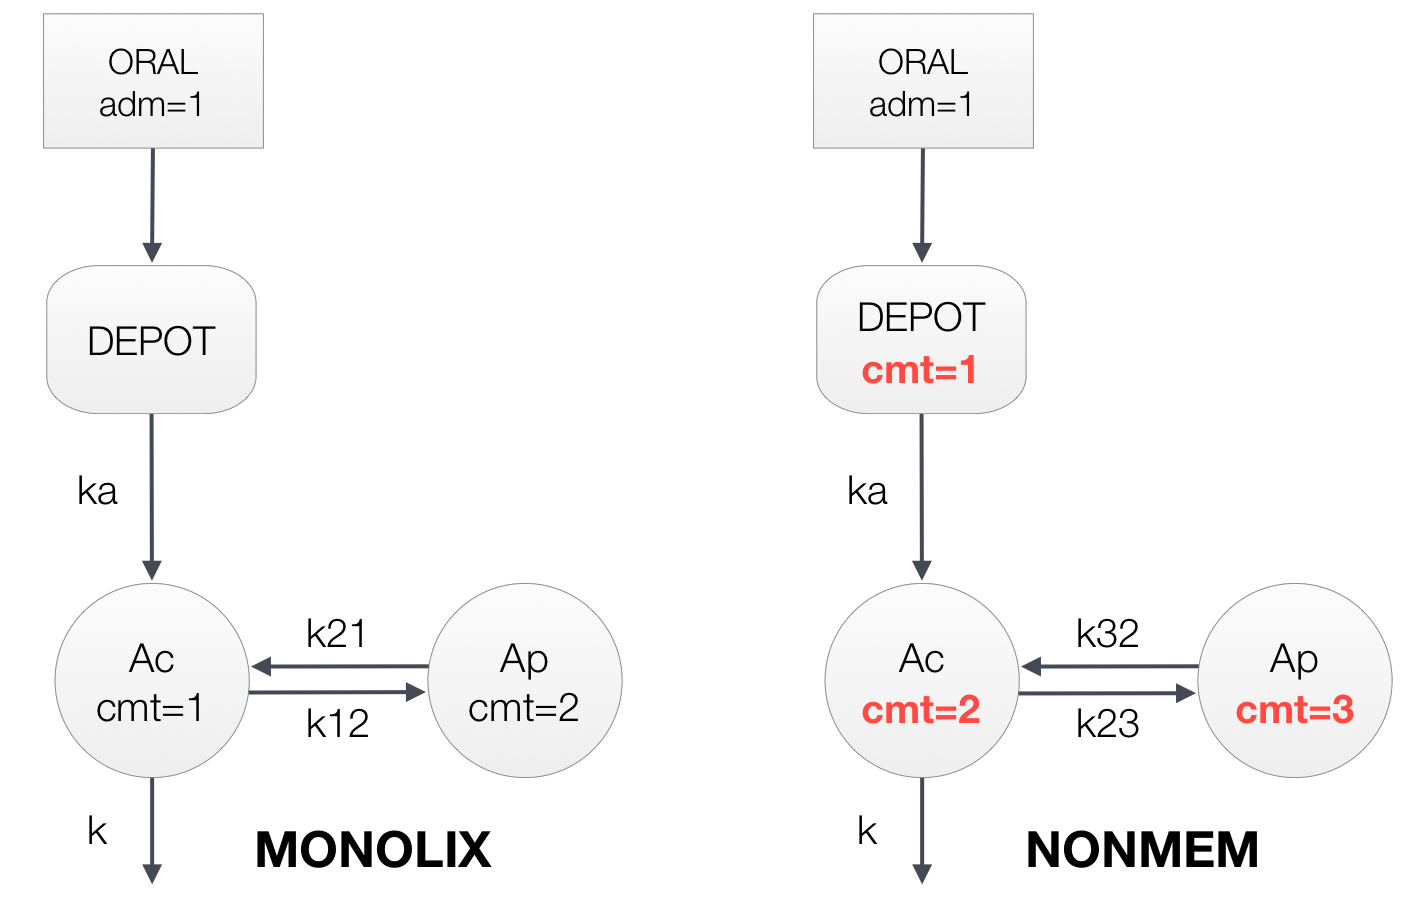
\includegraphics[width=110mm]{pics/Advan4}
\caption{ADVAN4 model, with compartment numbering dependent on the target tool. 
Note, that not only the compartment numbers are different in NONMEM coded model, 
the rate constants names are different as well.}
\label{fig:Advan4}
\end{figure}


\begin{table}[ht!]
\footnotesize
\parbox{.5\linewidth}{
\centering
\begin{tabular}{ccccc}
  \hline
   \multicolumn{5}{c}{\textbf{MONOLIX}} \\
  \hline
ID & TIME & AMT & \textbf{ADM} & Y \\
  \hline
1  & 0        & 10   & \textbf{1} & .       \\
1  & 2        & .      & . & 5        \\
... &  ...      &  ...   &  ...&  ...     \\
\end{tabular}
}
\hfill
\parbox{.5\linewidth}{
\centering
\begin{tabular}{ccccc}
  \hline
   \multicolumn{5}{c}{\textbf{NONMEM}} \\
  \hline
ID & TIME & AMT & \textbf{\textcolor{red}{CMT}} & DV \\
  \hline
1  & 0        & 10   & \textbf{\textcolor{red}{1}}   & .    \\
1  & 2        & .      & 2    & 5   \\
... &  ...      &  ...   &  ... & ...  \\
\end{tabular}
}
\caption{MONOLIX and NONMEM datasets for the ADVAN4 model.}
\end{table}

\begin{table}[h!]
\setlength{\tabcolsep}{15pt}
\begin{center}
%\begin{tabular*}{.95\textwidth}{@{\extracolsep{\fill} } ll}
\begin{tabular}{l}
  \hline \hline
PK macro  \\[-.25ex]
  \hline
\lstset{language=NONMEMdataSet}
\begin{lstlisting}
input = {ka, V, k, k12, k21}
PK:
compartment(cmt=1, amount=Ac, volume=V)
peripheral(k12, k21, amount=Ap)
oral(adm=1, cmt=1, ka)
elimination(cmt=1, k)
\end{lstlisting}
%&
%\lstset{language=NONMEMdataSet}
%\begin{lstlisting}
%input = {ka, V, k, k12, k21}
%PK:
%compartment(cmt=1, amount=Ac, volume=V)
%[*compartment(cmt=3, amount=Depot)*]
%peripheral(k12, k21, amount=Ap)
%oral(adm=1, [*fromCmt=3,*] cmt=1, ka)
%elimination(cmt=1, k)
%\end{lstlisting} 
\\
  \hline
\end{tabular}
\caption{PK macros  for the ADVAN4 model, as shown in Figure \ref{fig:Advan4} (left).}
\label{tab:advan4Table}
\end{center}
\end{table}


PharmML code:
\lstset{language=XML}
\begin{lstlisting}
        <StructuralModel blkId="sm4">
            <ct:Variable symbolType="real" symbId="Ac"/>
            <ct:Variable symbolType="real" symbId="Ap"/>
            <ct:Variable symbolType="real" symbId="Cc">
                <ct:Assign>
                    <math:Equation>
                        <math:Binop op="divide">
                            <ct:SymbRef symbIdRef="Ac"/>
                            <ct:SymbRef blkIdRef="pm1" symbIdRef="V"/>
                        </math:Binop>
                    </math:Equation>
                </ct:Assign>
            </ct:Variable>
            
            <PKmacros>
                <Compartment>
                    <Value argument="cmt">
                        <ct:Int>1</ct:Int>
                    </Value>
                    <Value argument="amount">
                        <ct:SymbRef symbIdRef="Ac"/>
                    </Value>
                    <Value argument="volume">
                        <ct:SymbRef blkIdRef="pm1" symbIdRef="V"/>
                    </Value>
                </Compartment>
                
                <Peripheral>
                    <Value>
                        <ct:SymbRef blkIdRef="pm1" symbIdRef="k12"/>
                    </Value>
                    <Value>
                        <ct:SymbRef blkIdRef="pm1" symbIdRef="k21"/>
                    </Value>
                    <Value argument="amount">
                        <ct:SymbRef symbIdRef="Ap"/>
                    </Value>
                </Peripheral>
                
                <Oral>
                    <Value argument="adm">
                        <ct:Int>1</ct:Int>
                    </Value>
                    <Value argument="cmt">
                        <ct:Int>1</ct:Int>
                    </Value>
                    <Value>
                        <ct:SymbRef blkIdRef="pm1" symbIdRef="ka"/>
                    </Value>
                </Oral>
                
                <Elimination>
                    <Value argument="cmt">
                        <ct:Int>1</ct:Int>
                    </Value>
                    <Value>
                        <ct:SymbRef blkIdRef="pm1" symbIdRef="k"/>
                    </Value>
                </Elimination>
            </PKmacros>
        </StructuralModel>
\end{lstlisting}


%\cleardoublepage
%%%%%%%%%%%%%%%%%%%%%%%%%%%%%%%%%%%%%%%%%%%%%%%%%%%%%%%%%%%%%%%%%%%%%%
\subsection{ADVAN10, TRANS1 -- 1-comp IV input with saturable elimination}
ODE formulation:
\begin{align}
\frac{dAc}{dt} &= - \frac{Vm \times Ac}{Km + Ac}  \nonumber
\end{align}

\begin{figure}[htbp!]
\centering
 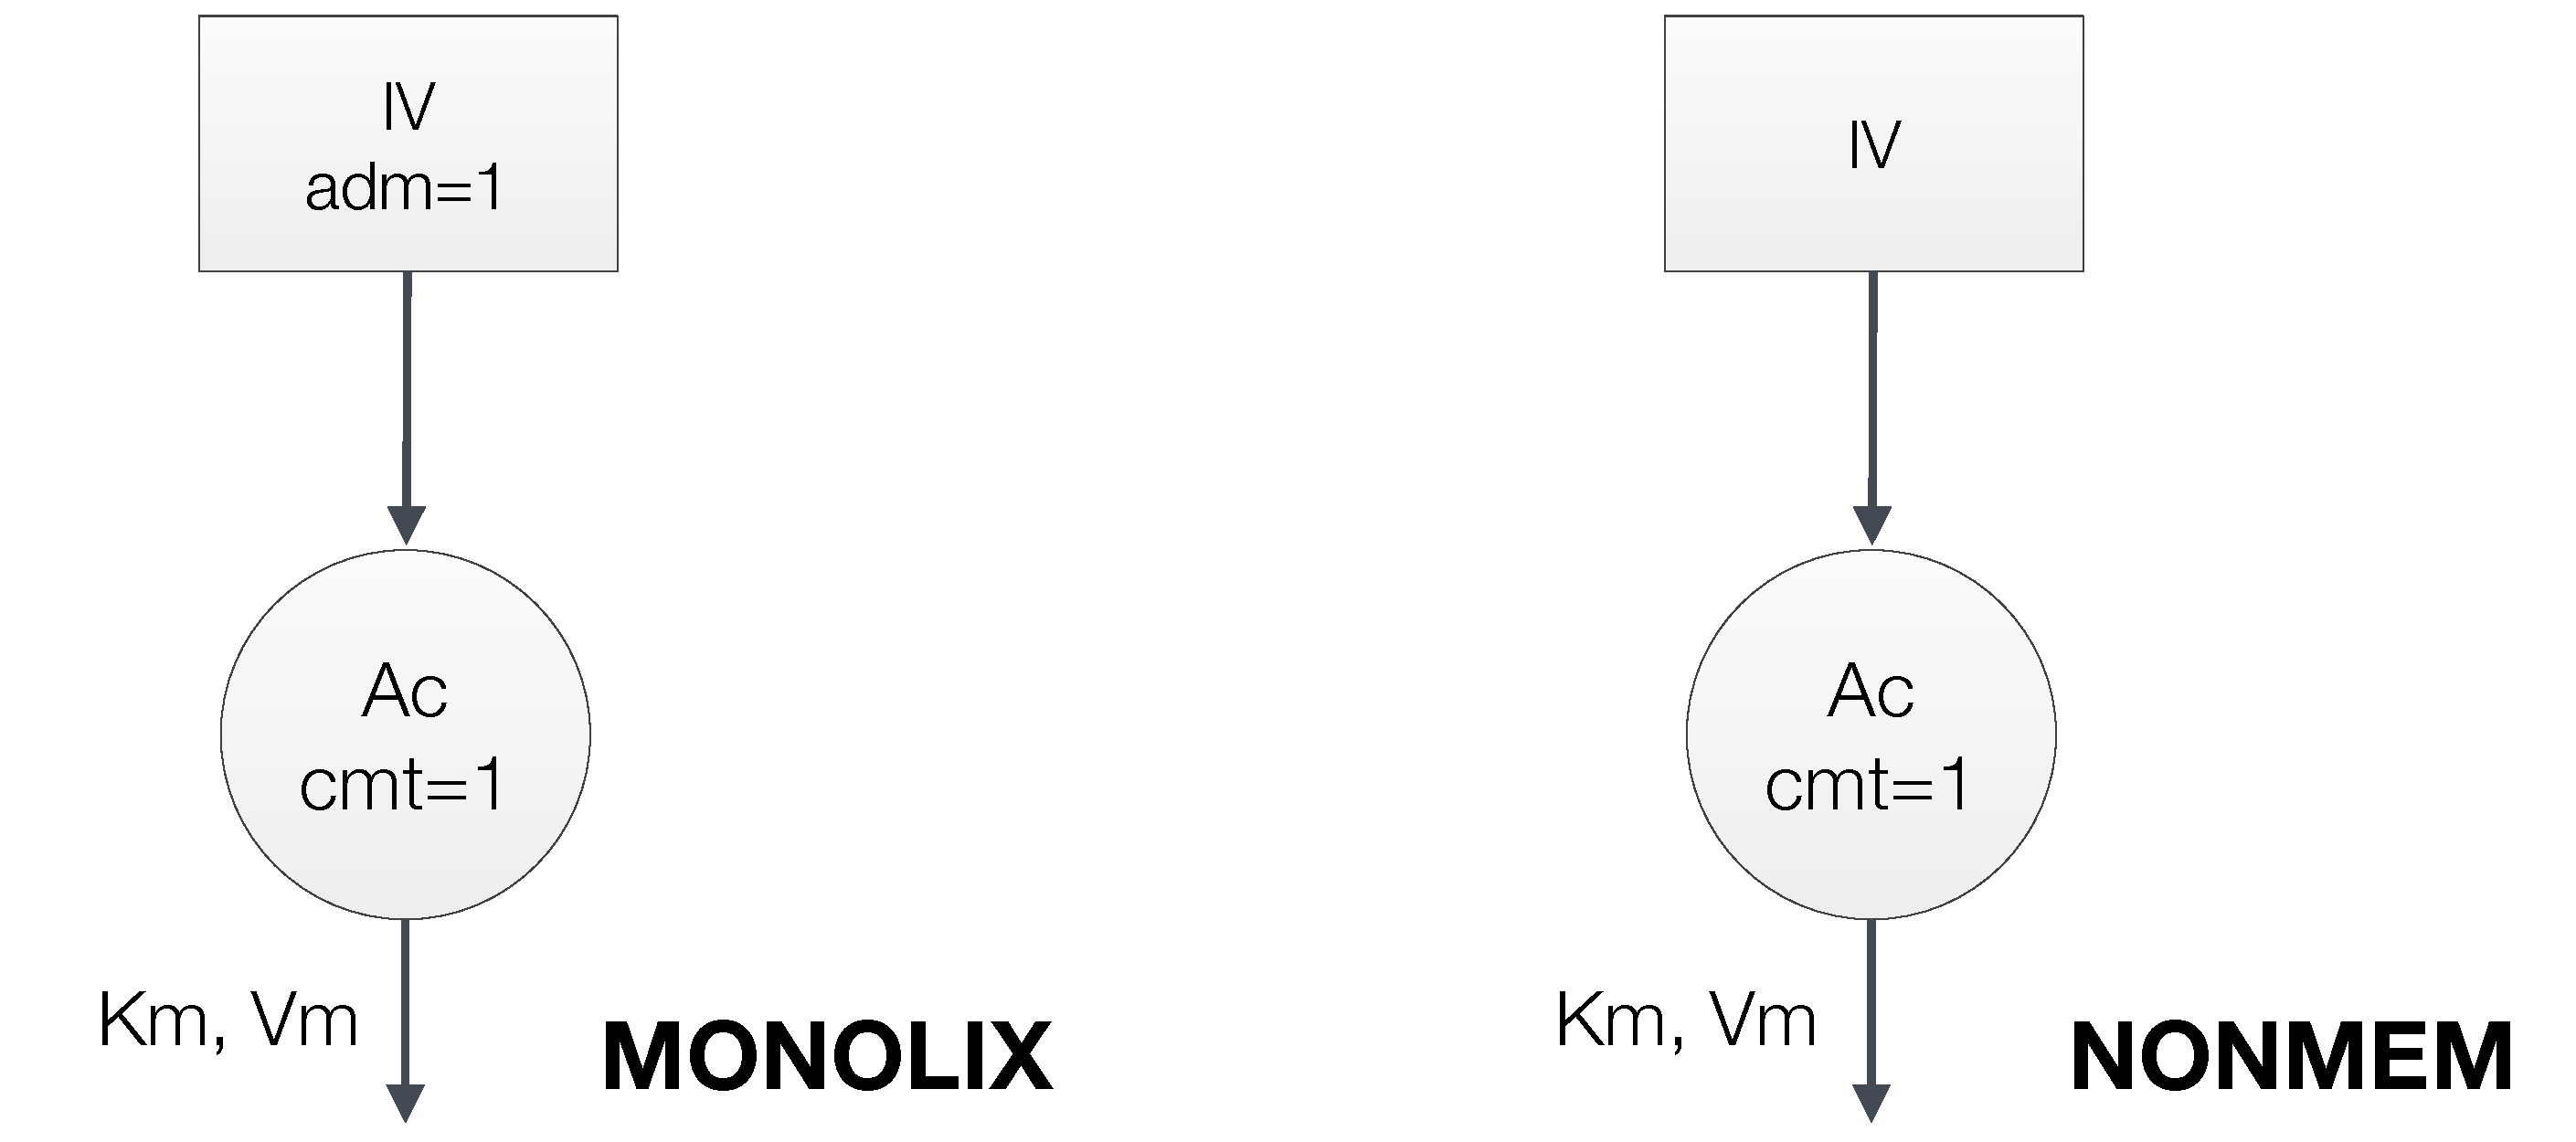
\includegraphics[width=100mm]{pics/Advan10}
\caption{ADVAN10 model, in this case compartment numbering is identical.}
\label{fig:Advan10}
\end{figure}


\begin{table}[ht!]
\footnotesize
\parbox{.5\linewidth}{
\centering
\begin{tabular}{ccccc}
  \hline
   \multicolumn{5}{c}{\textbf{MONOLIX}} \\
  \hline
ID & TIME & AMT & \textbf{ADM} & Y \\
  \hline
1  & 0        & 10   & \textbf{1} & .       \\
1  & 2        & .      &	.	& 5        \\
... &  ...      &  ...   &  ... &  ...     \\
\end{tabular}
}
\hfill
\parbox{.5\linewidth}{
\centering
\begin{tabular}{ccccc}
  \hline
   \multicolumn{5}{c}{\textbf{NONMEM}} \\
  \hline
ID & TIME & AMT & \textbf{CMT} & DV \\
  \hline
1  & 0        & 10   & \textbf{1}   & .    \\
1  & 2        & .      & 1    & 5   \\
... &  ...      &  ...   &  ... & ...  \\
\end{tabular}
}
\caption{MONOLIX and NONMEM datasets for the ADVAN10 model.}
\end{table}


\begin{table}[h!]
\setlength{\tabcolsep}{15pt}
\begin{center}
%\begin{tabular*}{.95\textwidth}{@{\extracolsep{\fill} } ll}
\begin{tabular}{l}
  \hline \hline
PK macro \\[-.25ex]
  \hline
\lstset{language=NONMEMdataSet}
\begin{lstlisting}
input = {V, Km, Vm}
PK:
compartment(cmt=1, amount=Ac, volume=V)
iv(adm=1, cmt=1)
elimination(cmt=1, Km, Vm)
\end{lstlisting}
%&
%\lstset{language=NONMEMdataSet}
%\begin{lstlisting}
%input = {V, Km, Vm}
%PK:
%compartment(cmt=1, amount=Ac, volume=V)
%iv(adm=1, cmt=1)
%elimination(cmt=1, Km, Vm)
%\end{lstlisting} 
\\
  \hline
\end{tabular}
\caption{PK macros for the ADVAN10 model, as shown in Figure \ref{fig:Advan10} (left).}
\label{tab:advan10Table}
\end{center}
\end{table}


PharmML code:
\lstset{language=XML}
\begin{lstlisting}
        <StructuralModel blkId="sm10">
            <ct:Variable symbolType="real" symbId="Ac"/>
            <ct:Variable symbolType="real" symbId="Cc">
                <ct:Assign>
                    <math:Equation>
                        <math:Binop op="divide">
                            <ct:SymbRef symbIdRef="Ac"/>
                            <ct:SymbRef blkIdRef="pm1" symbIdRef="V"/>
                        </math:Binop>
                    </math:Equation>
                </ct:Assign>
            </ct:Variable>
            
            <PKmacros>
                <Compartment>
                    <Value argument="cmt">
                        <ct:Int>1</ct:Int>
                    </Value>
                    <Value argument="amount">
                        <ct:SymbRef symbIdRef="Ac"/>
                    </Value>
                    <Value argument="volume">
                        <ct:SymbRef blkIdRef="pm1" symbIdRef="V"/>
                    </Value>
                </Compartment>
                
                <IV>
                    <Value argument="adm">
                        <ct:Int>1</ct:Int>
                    </Value>
                    <Value argument="cmt">
                        <ct:Int>1</ct:Int>
                    </Value>
                </IV>
                
                <Elimination>
                    <Value argument="cmt">
                        <ct:Int>1</ct:Int>
                    </Value>
                    <Value>
                        <ct:SymbRef blkIdRef="pm1" symbIdRef="Km"/>
                    </Value>
                    <Value>
                        <ct:SymbRef blkIdRef="pm1" symbIdRef="Vm"/>
                    </Value>
                </Elimination>
            </PKmacros>
        </StructuralModel>
\end{lstlisting}


%\cleardoublepage
%%%%%%%%%%%%%%%%%%%%%%%%%%%%%%%%%%%%%%%%%%%%%%%%%%%%%%%%%%%%%%%%%%%%%%
\subsection{ADVAN11, TRANS1 -- 3-comp IV input}
\label{subsubsec:ADVAN11}
ODE formulation:
\begin{align} % placement: default is "center", options are "top" and "bottom"
\frac{dAc}{dt} & =  - k_{12} \times Ac + k_{21} \times Ap1- k_{13} \times Ac \nonumber \\
			& + k_{31} \times Ap2 - k \times Ac  \nonumber \\
\frac{dAp1}{dt} & =  k_{12} \times Ac - k_{21} \times Ap1  \nonumber \\
\frac{dAp2}{dt} & =  k_{13} \times Ac - k_{31} \times Ap2  \nonumber
\end{align} 


\begin{figure}[htbp!]
\centering
 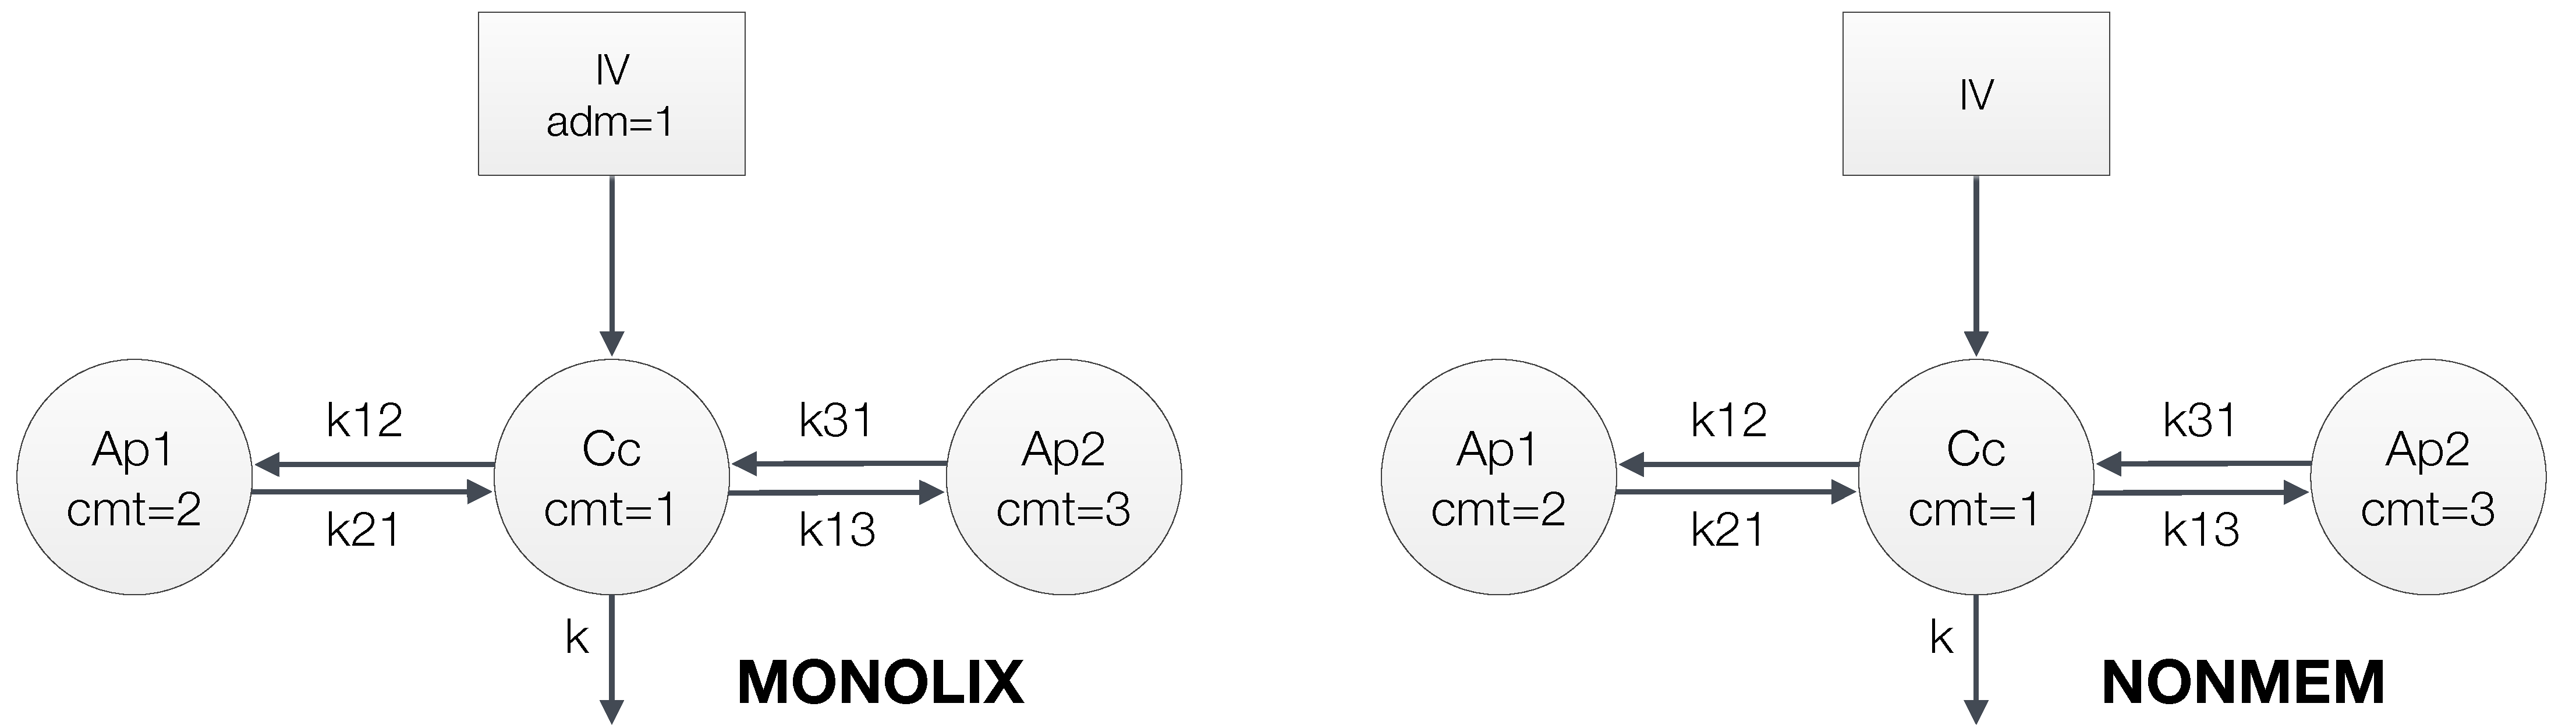
\includegraphics[width=160mm]{pics/Advan11}
\caption{ADVAN11 model, in this case compartment numbering is identical.}
\label{fig:Advan11}
\end{figure}


\begin{table}[ht!]
\footnotesize
\parbox{.5\linewidth}{
\centering
\begin{tabular}{ccccc}
  \hline
   \multicolumn{5}{c}{\textbf{MONOLIX}} \\
  \hline
ID & TIME & AMT & \textbf{ADM} & Y \\
  \hline
1  & 0        & 10   & \textbf{1} & .       \\
1  & 2        & .      & . 	& 5        \\
... &  ...      &  ...   &  ...   &  ...    \\
\end{tabular}
}
\hfill
\parbox{.5\linewidth}{
\centering
\begin{tabular}{ccccc}
  \hline
   \multicolumn{5}{c}{\textbf{NONMEM}} \\
  \hline
ID & TIME & AMT & \textbf{CMT} & DV \\
  \hline
1  & 0        & 10   & \textbf{1}   & .    \\
1  & 2        & .      & 1    & 5   \\
... &  ...      &  ...   &  ... & ...  \\
\end{tabular}
}
\caption{MONOLIX and NONMEM datasets for the ADVAN11 model.}
\end{table}


\begin{table}[h!]
\setlength{\tabcolsep}{15pt}
\begin{center}
%\begin{tabular*}{.95\textwidth}{@{\extracolsep{\fill} } ll}
\begin{tabular}{c}
  \hline \hline
PK macro \\[-.25ex]
  \hline
\lstset{language=NONMEMdataSet}
\begin{lstlisting}
input = {V, k, k12, k21, k13, k31}
PK:
compartment(cmt=1, amount=Ac, volume=V)
peripheral(k12, k21, amount=Ap1)
peripheral(k13, k31, amount=Ap2)
iv(adm=1, cmt=1)
elimination(cmt=1, k)
\end{lstlisting}
%&
%\lstset{language=NONMEMdataSet}
%\begin{lstlisting}
%input = {V, k, k12, k21, k13, k31}
%PK:
%compartment(cmt=1, amount=Ac, volume=V)
%peripheral(k12, k21, amount=Ap1)
%peripheral(k13, k31, amount=Ap2)
%iv(adm=1, cmt=1)
%elimination(cmt=1, k)
%\end{lstlisting} 
\\
  \hline
\end{tabular}
\caption{PK macros  for the ADVAN11 model, as shown in Figure \ref{fig:Advan11} (left).}
\label{tab:advan11Table}
\end{center}
\end{table}


PharmML code:
\lstset{language=XML}
\begin{lstlisting}
        <StructuralModel blkId="sm11">
            <ct:Variable symbolType="real" symbId="Ac"/>
            <ct:Variable symbolType="real" symbId="Ap1"/>
            <ct:Variable symbolType="real" symbId="Ap2"/>
            <ct:Variable symbolType="real" symbId="Cc">
                <ct:Assign>
                    <math:Equation>
                        <math:Binop op="divide">
                            <ct:SymbRef symbIdRef="Ac"/>
                            <ct:SymbRef blkIdRef="pm1" symbIdRef="V"/>
                        </math:Binop>
                    </math:Equation>
                </ct:Assign>
            </ct:Variable>
            
            <PKmacros>
                <Compartment>
                    <Value argument="cmt">
                        <ct:Int>1</ct:Int>
                    </Value>
                    <Value argument="amount">
                        <ct:SymbRef symbIdRef="Ac"/>
                    </Value>
                    <Value argument="volume">
                        <ct:SymbRef blkIdRef="pm1" symbIdRef="V"/>
                    </Value>
                </Compartment>
                
                <Peripheral>
                    <Value>
                        <ct:SymbRef blkIdRef="pm1" symbIdRef="k12"/>
                    </Value>
                    <Value>
                        <ct:SymbRef blkIdRef="pm1" symbIdRef="k21"/>
                    </Value>
                    <Value argument="amount">
                        <ct:SymbRef symbIdRef="Ap1"/>
                    </Value>
                </Peripheral>
                
                <Peripheral>
                    <Value>
                        <ct:SymbRef blkIdRef="pm1" symbIdRef="k13"/>
                    </Value>
                    <Value>
                        <ct:SymbRef blkIdRef="pm1" symbIdRef="k31"/>
                    </Value>
                    <Value argument="amount">
                        <ct:SymbRef symbIdRef="Ap2"/>
                    </Value>
                </Peripheral>
                
                <IV>
                    <Value argument="adm">
                        <ct:Int>1</ct:Int>
                    </Value>
                    <Value argument="cmt">
                        <ct:Int>1</ct:Int>
                    </Value>
                </IV>
                
                <Elimination>
                    <Value argument="cmt">
                        <ct:Int>1</ct:Int>
                    </Value>
                    <Value>
                        <ct:SymbRef blkIdRef="pm1" symbIdRef="k"/>
                    </Value>
                </Elimination>
            </PKmacros>
        </StructuralModel>
\end{lstlisting}


%\cleardoublepage
%%%%%%%%%%%%%%%%%%%%%%%%%%%%%%%%%%%%%%%%%%%%%%%%%%%%%%%%%%%%%%%%%%%%%%
\subsection{ADVAN12, TRANS1 -- 3-comp 1st order input}
\label{subsubsec:ADVAN12}
ODE formulation:
\begin{align}
\frac{dAd}{dt} & =  -ka \times Ad \nonumber \\
\frac{dAc}{dt} & = ka \times Ad - k_{12} \times Ac + k_{21} \times Ap1 - k_{13} \times Ac \nonumber \\
			& + k_{31} \times Ap2 - k \times Ac  \nonumber \\
\frac{dAp1}{dt} & =  k_{12} \times Ac - k_{21} \times Ap1  \nonumber \\
\frac{dAp2}{dt} & =  k_{13} \times Ac - k_{31} \times Ap2  \nonumber
\end{align}

\begin{figure}[htbp!]
\centering
 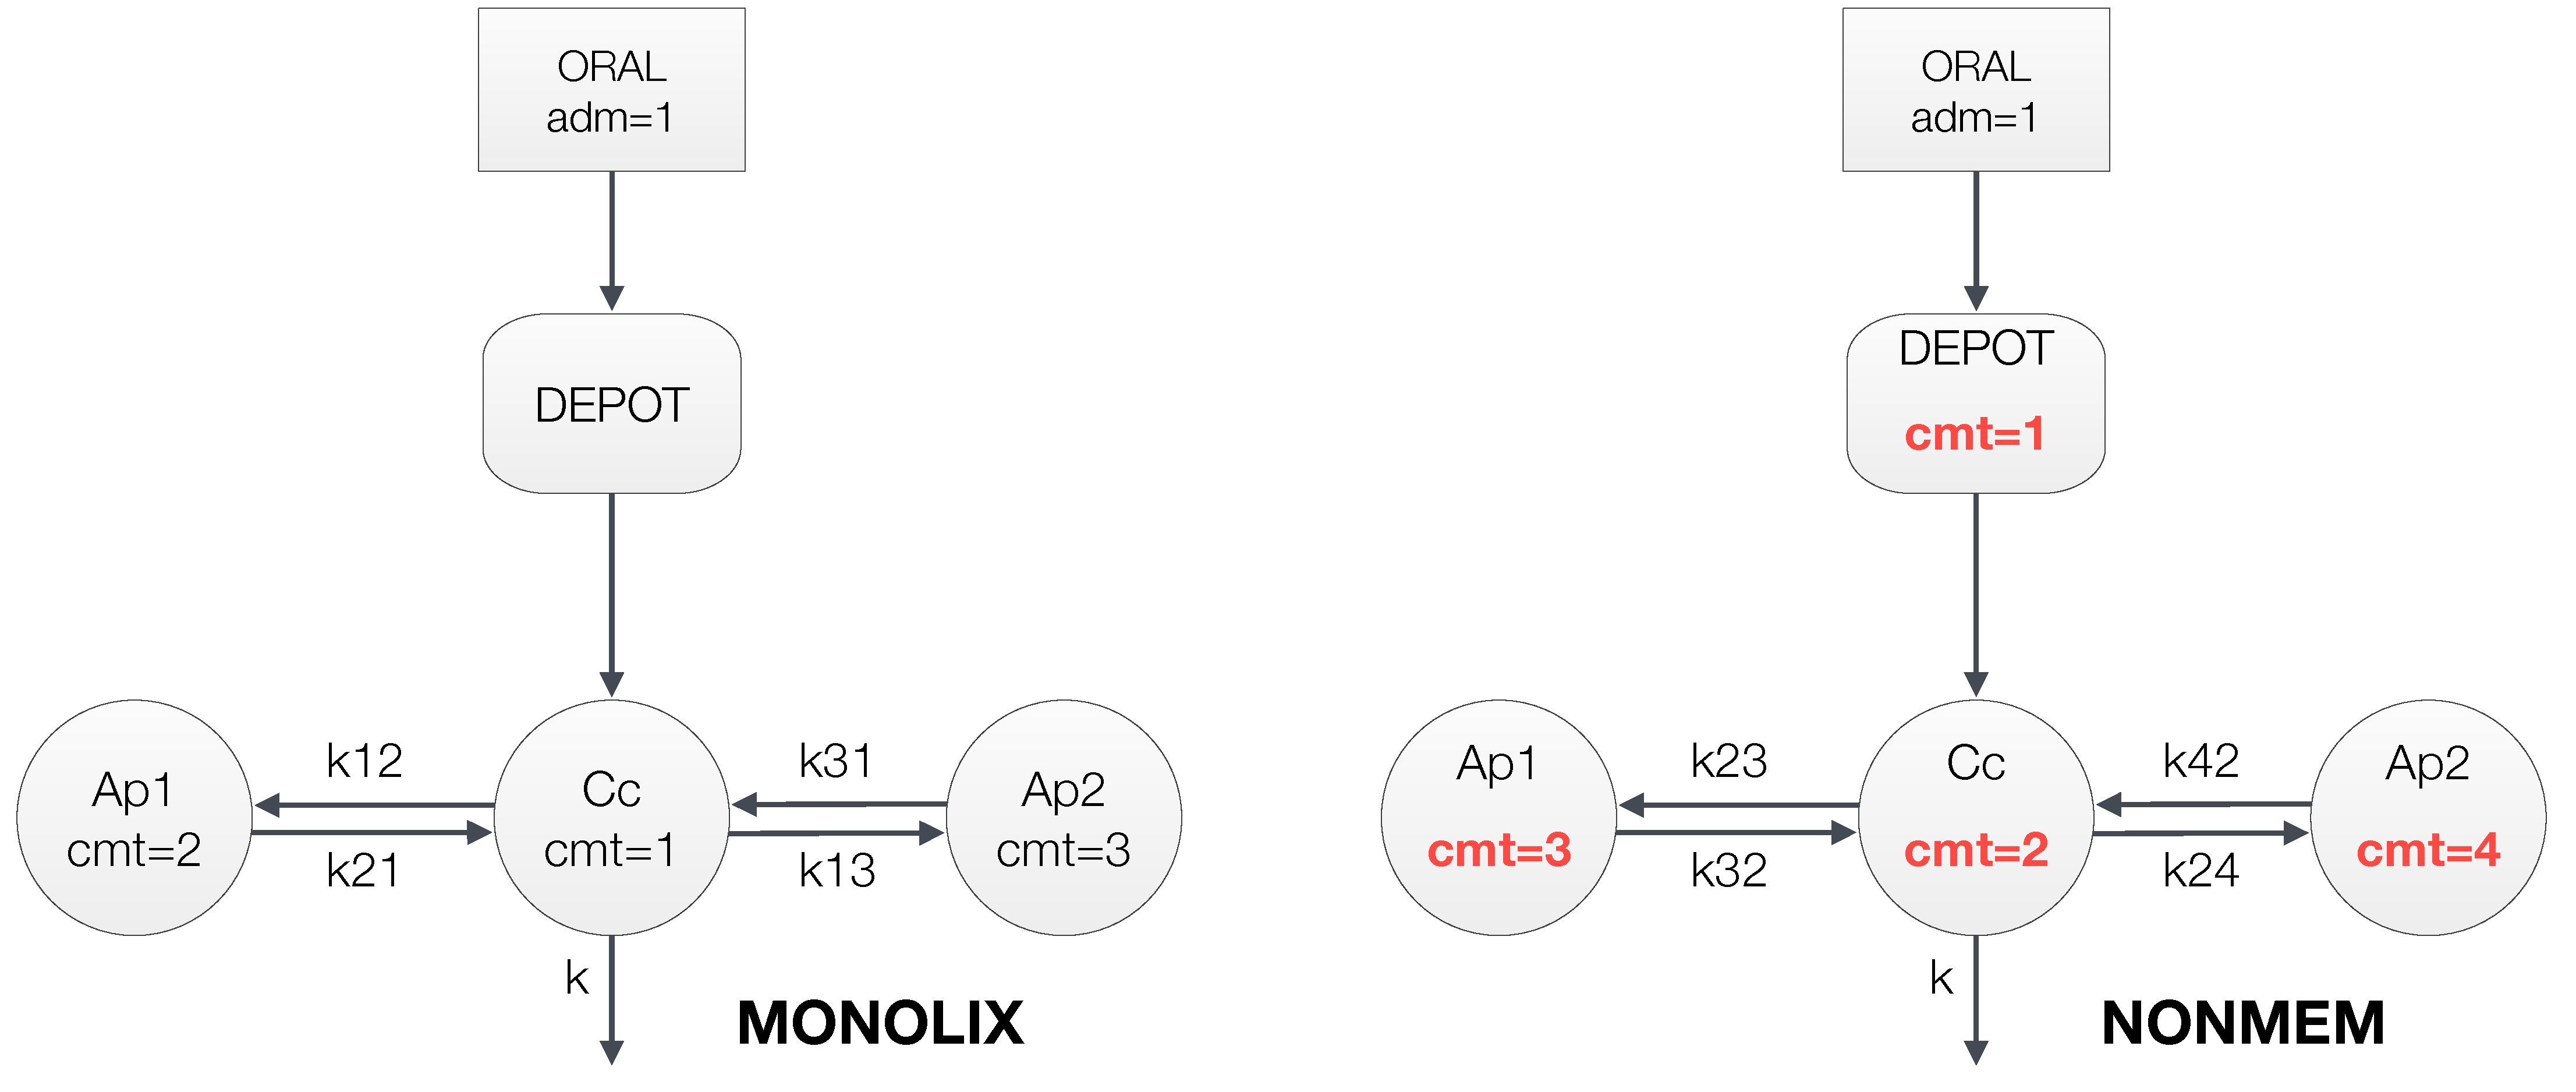
\includegraphics[width=160mm]{pics/Advan12}
\caption{ADVAN12 model, with compartment numbering dependent on the target tool. 
Note, that not only the compartment numbers are different in NONMEM coded model, 
the rate constants names are different as well.}
\label{fig:Advan12}
\end{figure}


\begin{table}[ht!]
\footnotesize
\parbox{.5\linewidth}{
\centering
\begin{tabular}{ccccc}
  \hline
   \multicolumn{5}{c}{\textbf{MONOLIX}} \\
  \hline
ID & TIME & AMT & \textbf{ADM} & Y \\
  \hline
1  & 0        & 10   & \textbf{1} & .       \\
1  & 2        & .      & . 	& 5        \\
... &  ...      &  ...   &  ...  &  ...     \\
\end{tabular}
}
\hfill
\parbox{.5\linewidth}{
\centering
\begin{tabular}{ccccc}
  \hline
   \multicolumn{5}{c}{\textbf{NONMEM}} \\
  \hline
ID & TIME & AMT & \textbf{\textcolor{red}{CMT}} & DV \\
  \hline
1  & 0        & 10   & \textbf{\textcolor{red}{1}}   & .    \\
1  & 2        & .      & 2    & 5   \\
... &  ...      &  ...   &  ... & ...  \\
\end{tabular}
}
\caption{MONOLIX and NONMEM datasets for the ADVAN12 model.}
\end{table}


\begin{table}[h!]
\setlength{\tabcolsep}{15pt}
\begin{center}
%\begin{tabular*}{.95\textwidth}{@{\extracolsep{\fill} } ll}
\begin{tabular}{l}
  \hline \hline
PK macro \\[-.25ex]
  \hline
\lstset{language=NONMEMdataSet}
\begin{lstlisting}
input = {ka, V, k, k12, k21, k13, k31}
PK:
compartment(cmt=1, amount=Ac, volume=V)
peripheral(k12, k21, amount=Ap1)
peripheral(k13, k31, amount=Ap2)
oral(adm=1, cmt=1, ka)
elimination(cmt=1, k)
\end{lstlisting}
\\
  \hline
\end{tabular}
\caption{PK macros  for the ADVAN12 model, as shown in Figure \ref{fig:Advan12} (left).}
\label{tab:advan12Table}
\end{center}
\end{table}


PharmML code:
\lstset{language=XML}
\begin{lstlisting}
        <StructuralModel blkId="sm12">
            <ct:Variable symbolType="real" symbId="Ac"/>
            <ct:Variable symbolType="real" symbId="Ap1"/>
            <ct:Variable symbolType="real" symbId="Ap2"/>
            <ct:Variable symbolType="real" symbId="Cc">
                <ct:Assign>
                    <math:Equation>
                        <math:Binop op="divide">
                            <ct:SymbRef symbIdRef="Ac"/>
                            <ct:SymbRef blkIdRef="pm1" symbIdRef="V"/>
                        </math:Binop>
                    </math:Equation>
                </ct:Assign>
            </ct:Variable>
            
            <PKmacros>
                <Compartment>
                    <Value argument="cmt">
                        <ct:Int>1</ct:Int>
                    </Value>
                    <Value argument="amount">
                        <ct:SymbRef symbIdRef="Ac"/>
                    </Value>
                    <Value argument="volume">
                        <ct:SymbRef blkIdRef="pm1" symbIdRef="V"/>
                    </Value>
                </Compartment>
                
                <Peripheral>
                    <Value>
                        <ct:SymbRef blkIdRef="pm1" symbIdRef="k12"/>
                    </Value>
                    <Value>
                        <ct:SymbRef blkIdRef="pm1" symbIdRef="k21"/>
                    </Value>
                    <Value argument="amount">
                        <ct:SymbRef symbIdRef="Ap1"/>
                    </Value>
                </Peripheral>
                
                <Peripheral>
                    <Value>
                        <ct:SymbRef blkIdRef="pm1" symbIdRef="k13"/>
                    </Value>
                    <Value>
                        <ct:SymbRef blkIdRef="pm1" symbIdRef="k31"/>
                    </Value>
                    <Value argument="amount">
                        <ct:SymbRef symbIdRef="Ap2"/>
                    </Value>
                </Peripheral>
                
                <Oral>
                    <Value argument="adm">
                        <ct:Int>1</ct:Int>
                    </Value>
                    <Value argument="cmt">
                        <ct:Int>1</ct:Int>
                    </Value>
                    <Value>
                        <ct:SymbRef blkIdRef="pm1" symbIdRef="ka"/>
                    </Value>
                </Oral>
                
                <Elimination>
                    <Value argument="cmt">
                        <ct:Int>1</ct:Int>
                    </Value>
                    <Value>
                        <ct:SymbRef blkIdRef="pm1" symbIdRef="k"/>
                    </Value>
                </Elimination>
            </PKmacros>
        </StructuralModel>
\end{lstlisting}

%
%\begin{table}[ht!]
%\setlength{\tabcolsep}{5pt}
%\begin{center}
%\begin{tabular}{ll}
%  \hline
%PK macro 	& PharmML  \\
%  \hline
%%			\multicolumn{2}{c}{Mapping in a \xelem{CategoricalData} model}  \\  [.5ex]
%  \hline
%\lstset{language=XML}
%\begin{lstlisting}
%
%\end{lstlisting}
%&
%\lstset{language=XML}
%\begin{lstlisting}
%
%\end{lstlisting}
%\\
%    \hline
%\end{tabular}
%\caption{Code...}
%\label{tab:exampleXYZ}
%\end{center}
%\end{table}


%%\cleardoublepage
%\subsection{Pavia Whiteboard}
%
%\begin{figure}[htb!]
%\centering
%  \includegraphics[width=130mm]{pics/Pavia1}
% \caption{Blackboard with forcing function discussion.}
% \label{Pavia1}
%\end{figure}


% {\color{red} \scshape{NEW}}
%\cleardoublepage
%%%%%%%%%%%%%%%%%%%%%%%%%%%%%%%%%%%%%%%%%%%%%%%%%%%%%%%
\section{Alternative model parameterizations}

In case of routine others then the default TRANS1 the procedure is quite straightforward. 
The reparametrization, called \emph{Reparameterization Lines} in the NONMEM manual
\cite{NONMEM:2009}, can be defined in the \xelem{ParameterModel} leaving the PK macros in the 
\xelem{StructuralModel} unchanged. This is presented using the basic ADVAN1 and more 
complex ADVAN11 routines.

\subsection{ADVAN1 with TRANS2}
Following table shows the two allowed parameterizations for ADVAN1 and the according formula. 
\begin{table}[ht]
\begin{center}
\begin{tabular*}{.8\textwidth}{@{\extracolsep{\fill} } lll}
  \hline
  \hline
  TRANS1								& TRANS2						& Formula \\
  \hline
K Rate constant of elimination				& CL Clearance 					& K=CL/V \\
									& V Volume of distribution				& \\
\end{tabular*}
\caption{ADVAN1 parameters with TRANS1 and TRANS2.}
\end{center}
\end{table}

Table \ref{tab:ADVAN1TRANS1reparameterisation} shows the PK macros for the two options
\begin{table}[ht]
\begin{center}
\begin{tabular*}{.8\textwidth}{@{\extracolsep{\fill} } ll}
  \hline
  \hline
ADVAN1, TRANS1 & ADVAN1, TRANS4 \\
  \hline
\lstset{language=NONMEMdataSet}
\begin{lstlisting}
compartment(cmt=1, amount=Ac, volume=V)
iv(cmt=1)
elimination(cmt=1, k)
\end{lstlisting}
&
\lstset{language=NONMEMdataSet}
\begin{lstlisting}
compartment(cmt=1, amount=Ac, volume=V)
iv(cmt=1)
elimination(cmt=1, k=CL/V)
\end{lstlisting}

\end{tabular*}
\caption{PK macros for ADVAN1 using two different parameterizations.}
\label{tab:ADVAN1TRANS1reparameterisation}
\end{center}
\end{table}

\paragraph{Version 1}
PharmML code -- modified from section \ref{subsubsec:ADVAN1}. The reparameterization is done in 
the parameter model \xatt{pm1}:
\lstset{language=XML}
\begin{lstlisting}

        <ParameterModel blkId="pm1">
            
            <!-- Reparameterization Lines for k, CL, V -->
            <SimpleParameter symbId="k">
                <ct:Assign>
                    <math:Equation>
                        <math:Binop op="divide">
                            <ct:SymbRef symbIdRef="CL"/>
                            <ct:SymbRef symbIdRef="V"/>
                        </math:Binop>
                    </math:Equation>
                </ct:Assign>
            </SimpleParameter>
            
        </ParameterModel>

        <StructuralModel blkId="sm1">
            <ct:Variable symbolType="real" symbId="Ac"/>
            <PKmacros>
                    <!-- omitted, identical to ADVAN1, TRANS1 -->
            </PKmacros>
        </StructuralModel>
\end{lstlisting}

\paragraph{Version 2}
PharmML code -- with reparameterization within macros:
\lstset{language=XML}
\begin{lstlisting}
        <StructuralModel blkId="sm1b">
            <ct:Variable symbolType="real" symbId="Ac"/>
            <ct:Variable symbolType="real" symbId="Cc">
                <!-- omitted details -->
            </ct:Variable>
            
            <PKmacros>
                <!-- omitted details -->
                
                <Elimination>
                    <Value argument="cmt">
                        <ct:Int>1</ct:Int>
                    </Value>
                    <Value argument="k">
                        <ct:Assign>
                            <math:Equation>
                                <math:Binop op="divide">
                                    <ct:SymbRef blkIdRef="pm1" symbIdRef="CL"/>
                                    <ct:SymbRef blkIdRef="pm1" symbIdRef="V"/>
                                </math:Binop>
                            </math:Equation>
                        </ct:Assign>
                    </Value>
                </Elimination>
            </PKmacros>
        </StructuralModel>
\end{lstlisting}


\subsection{ADVAN11 with TRANS4}
Following table shows the two allowed parameterizations for ADVAN11 and the according 
re-parameterisation formulas. 
\begin{table}[ht]
\begin{center}
\begin{tabular*}{.95\textwidth}{@{\extracolsep{\fill} } lll}
  \hline
  \hline
  TRANS1								& TRANS4						& Formula \\
  \hline
K Rate constant of elimination				& CL Clearance 					& K=CL/V1 \\
K12 Rate constant from central to periph. 1	& V1 Central volume  				& K12=Q2/V1 \\
K21 Rate constant from periph. 1 to central	& Q2 Intercompartmental clearance 1  	& K21=Q2/V2 \\
K13 Rate constant from central to periph. 2	& V2 Peripheral volume 1  			& K13=Q3/V1 \\
K31 Rate constant from periph. 2 to central	& Q3 Intercompartmental clearance 2  	& K31=Q3/V3 \\
									& V3 Peripheral volume 2  			& V3=V3 \\
\end{tabular*}
\caption{ADVAN11 parameters with TRANS1 and TRANS4.}
\end{center}
\end{table}
and the following table shows the PK macros for the two routines

\begin{table}[ht]
\begin{center}
\begin{tabular*}{.95\textwidth}{@{\extracolsep{\fill} } ll}
  \hline
  \hline
ADVAN11, TRANS1 & ADVAN11, TRANS4 \\
  \hline

\lstset{language=NONMEMdataSet}
\begin{lstlisting}
compartment(cmt=1, amount=Ac, volume=V)
peripheral(k12, k21, amount=Ap1)
peripheral(k13, k31, amount=Ap2)
iv(cmt=1)
elimination(cmt=1, k)
\end{lstlisting}
&
\lstset{language=NONMEMdataSet}
\begin{lstlisting}
compartment(cmt=1, amount=Ac, volume=V3)
peripheral(k12 = Q2/V1, k21 = Q2/V2, amount=Ap1)
peripheral(k13 = Q3/V1, k31 = Q3/V3, amount=Ap2)
iv(cmt=1)
elimination(cmt=1, k = CL/V1)
\end{lstlisting}

\end{tabular*}
\caption{PK macros for ADVAN11 using two different parameterizations.}
\end{center}
\end{table}

\paragraph{Version 1}
PharmML code -- modified from section \ref{subsubsec:ADVAN11}. In this case the 
reparameterization is done in the parameter model \xatt{pm1}, here example for one 
parameter:
\lstset{language=XML}
\begin{lstlisting}
        <ParameterModel blkId="pm1">
            
            <!-- Reparameterization Lines for k12, Q, V1 -->
            <SimpleParameter symbId="k12">
                <ct:Assign>
                    <math:Equation>
                        <math:Binop op="divide">
                            <ct:SymbRef symbIdRef="Q2"/>
                            <ct:SymbRef symbIdRef="V1"/>
                        </math:Binop>
                    </math:Equation>
                </ct:Assign>
            </SimpleParameter>
            <!-- omitted parameters k21, k13, k31 & V3 -->
            
        </ParameterModel>

        <StructuralModel blkId="sm1">
            <ct:Variable symbolType="real" symbId="Ac"/>
            <ct:Variable symbolType="real" symbId="Ap1"/>
            <ct:Variable symbolType="real" symbId="Ap2"/>
            <PKmacros>
                    <!-- omitted, identical to ADVAN11, TRANS1 -->
            </PKmacros>
        </StructuralModel>
\end{lstlisting}

\paragraph{Version 2}
PharmML code -- with reparameterization within macros:
\lstset{language=XML}
\begin{lstlisting}
        <ParameterModel blkId="pm1">
            
            <!-- Q2 -->
            <IndividualParameter symbId="Q2">
                <!-- omitted details -->
            </IndividualParameter>
            
            <!-- V1 -->
            <IndividualParameter symbId="V1">
                <!-- omitted details -->
            </IndividualParameter>
            
            <!-- V2 -->
            <IndividualParameter symbId="V2">
                <!-- omitted details -->
            </IndividualParameter>
            
            <!-- omitted other parameters Q3, V3, CL -->
            
        </ParameterModel>

        <StructuralModel blkId="sm1">
            <ct:Variable symbolType="real" symbId="Ac"/>
            <ct:Variable symbolType="real" symbId="Ap1"/>
            <ct:Variable symbolType="real" symbId="Ap2"/>
            <PKmacros>
            
                <!-- omitted other macros -->

                <Peripheral>
                    <Value argument="k12">
                        <ct:Assign>
                            <math:Equation>
                                <math:Binop op="divide">
                                    <ct:SymbRef blkIdRef="pm1" symbIdRef="Q2"/>
                                    <ct:SymbRef blkIdRef="pm1" symbIdRef="V1"/>
                                </math:Binop>
                            </math:Equation>
                        </ct:Assign>
                    </Value>
                    <Value argument="k21">
                        <ct:Assign>
                            <math:Equation>
                                <math:Binop op="divide">
                                    <ct:SymbRef blkIdRef="pm1" symbIdRef="Q2"/>
                                    <ct:SymbRef blkIdRef="pm1" symbIdRef="V2"/>
                                </math:Binop>
                            </math:Equation>
                        </ct:Assign>
                    </Value>
                    <Value argument="amount">
                        <ct:SymbRef symbIdRef="Ap1"/>
                    </Value>
                </Peripheral>

                <!-- omitted other macros -->
            </PKmacros>
        </StructuralModel>
\end{lstlisting}



%%%%%%%%%%%%%%%%%%%%%%%%%%%%%%%%%%%%%%%%%%%%%%%%%%%%%%%
\section{Complex PK macro examples}
Additional examples have been encoded in PharmML in order to further validate the schema
and to test the implementation of more complex PK macros.

\textbf{Note} that the first two of the following models, C1 (versions C1a and C1b) and C2, 
can be treated as equivalent to that discussed in Sections \ref{subsubsec:advan2}, 
\ref{subsubsec:ADVAN12}, and modelled by the ADVAN2 ands ADVAN12 routines, 
respectively, with an additional IV administration.

Importantly, \marginpar{\HandCuffLeft} the according dataset transformation reduces 
to the renaming of the ADM and CMT columns \textbf{but} only if the oral administration 
is treated as the first one, i.e. with attribute \xatt{adm=1}. Otherwise a renumbering 
is required as well. Examples C1a and C1b illustrate this.

%\cleardoublepage
%%%%%%%%%%%%%%%%%%%%%%%%%%%%%%%%%%%%%%%%%%%%%%%%%%%%%%%
\subsection{Example C1a}
%The following example is from \cite{Monolix4.3Tutorial:2014}, page 70. Here the original description
%(with referrences to the MONOLIX dataset format suing \xatt{adm} instead of \xatt{cmt}
%column, see below):
%"An additional column \xatt{adm} is used to specify the different types of administration.
%Here, \xatt{adm=1} indicates an oral administration and \xatt{adm=2} an IV bolus administration.
%The datafile only contains information about the administration, not about the absorption 
%process which will be described in the model."
The following example is from \cite{Monolix4.3Tutorial:2014}, pages 70-74. This model
can be modelled by the ADVAN2 routine, with an additional IV administration. Because the 
oral administration is labeled as the first one, attribute \xatt{adm=1}, no renumbering is required 
when transforming the data and renaming the ADM to CMT column is sufficient to get the suitable 
NONMEM data set.

\begin{figure}[htbp!]
\centering
 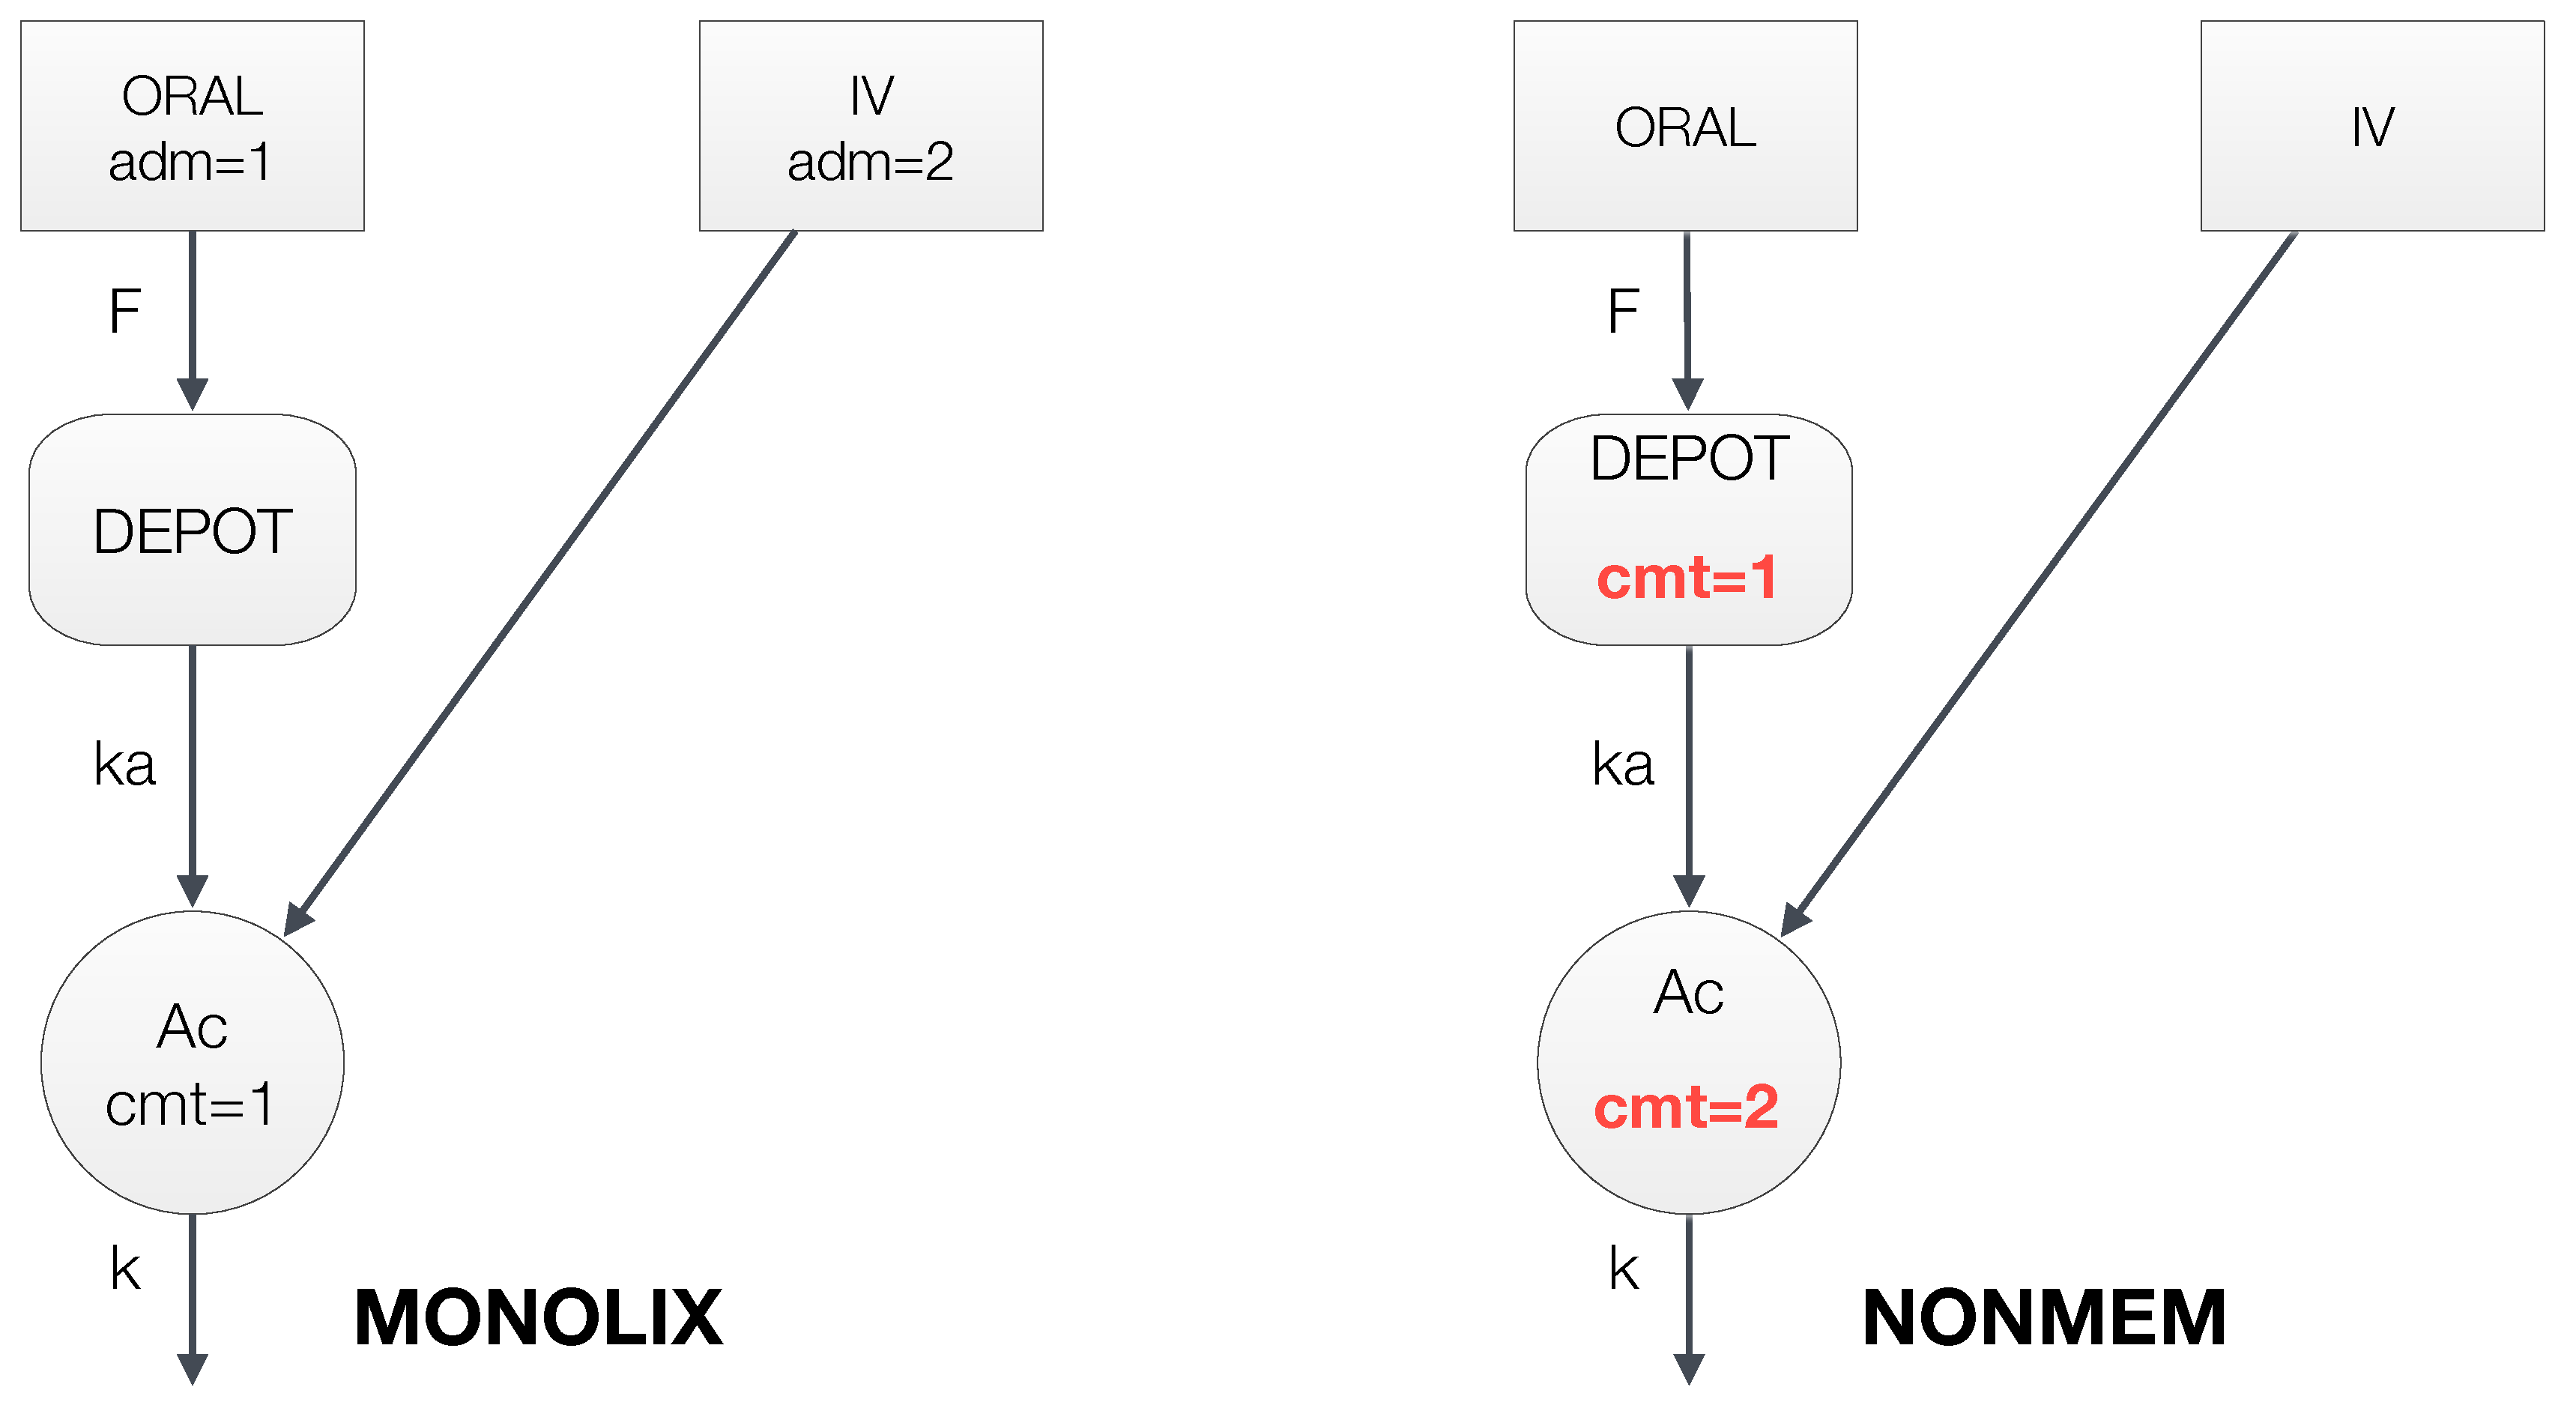
\includegraphics[width=120mm]{pics/ComplexModel1}
\caption{C1a model, with compartment numbering dependent on the target tool.}
\label{fig:ComplexModel1a}
\end{figure}

\begin{table}[ht!]
\footnotesize
\parbox{.5\linewidth}{
\centering
\begin{tabular}{ccccc}
  \hline
     \multicolumn{5}{c}{\textbf{MONOLIX}} \\
  \hline
ID	& TIME  & AMT	 & \textbf{ADM} &	Y \\
  \hline
1	& 0	    & 2.24	& \textbf{2}	& . \\
1	& 1	    & .	& .		 	& 142 \\
1	& 2	    & .	& .	 		& 54.9 \\
...     &  ...     &  ...     & ...  			& ...\\
1	& 6	    & 7	& \textbf{1}	& . \\
1	& 7	    & .	& .			& 192 \\
1	& 8	    & .	& .			& 141 \\
...     &  ...     &  ...     & ...  			& ...\\
2	& 0	    & 2.73	& \textbf{2}	& . \\
2	& 1	    & . 	& .			& 176 \\
...     &  ...     &  ...     & ...  			& ...\\
\end{tabular}
}
\hfill
\parbox{.5\linewidth}{
\centering
\begin{tabular}{ccccc}
  \hline
   \multicolumn{5}{c}{\textbf{NONMEM}} \\
  \hline
ID	& TIME  & AMT	 & \textbf{\textcolor{red}{CMT}} &	DV \\
  \hline
1	& 0	    & 2.24	& \textbf{\textcolor{red}{2}}	& . \\
1	& 1	    & .	& 2		 	& 142 \\
1	& 2	    & .	& 2	 		& 54.9 \\
...     &  ...     &  ...     & ...  			& ...\\
1	& 6	    & 7	& \textbf{\textcolor{red}{1}}	& . \\
1	& 7	    & .	& 2			& 192 \\
1	& 8	    & .	& 2			& 141 \\
...     &  ...     &  ...     & ...  			& ...\\
2	& 0	    & 2.73	& \textbf{\textcolor{red}{2}}	& . \\
2	& 1	    & . 	& 2	 		& 176 \\
...     &  ...     &  ...     & ...  			& ...\\
\end{tabular}
}
\caption{NONMEM and MONOLIX datasets for the C1a model. Because of the equivalence to 
ADVAN2 no renumbering is required when transforming the data and renaming the ADM 
to CMT column.}
\label{tab:C1aTable}
\end{table}

\begin{table}[h!]
\setlength{\tabcolsep}{15pt}
\begin{center}
\begin{tabular}{c}
%\begin{tabular*}{.95\textwidth}{@{\extracolsep{\fill} } ll}
  \hline \hline
PK macro  \\[-.25ex]
  \hline
\lstset{language=NONMEMdataSet}
\begin{lstlisting}
input = {F, ka, V, k}
PK:
compartment(cmt=1, amount=Ac)
oral(adm=1, cmt=1, ka, p=F)
iv(adm=2, cmt=1)
elimination(cmt=1, k)
Cc = Ac/V
\end{lstlisting}
%&
%\lstset{language=NONMEMdataSet}
%\begin{lstlisting}
%input = {F, ka, V, k}
%PK:
%compartment(cmt=1, amount=Ac)
%[*compartment(cmt=2, amount=Depot)*]
%oral(adm=1, [*fromCmt=2,*] cmt=1, ka, p=F)
%iv(adm=2, cmt=1)
%elimination(cmt=1, k)
%Cc = Ac/V
%\end{lstlisting} 
\\
  \hline
\end{tabular}
\caption{PK macros for the C1a model, as shown in Figure \ref{fig:ComplexModel1a} (left).}
\label{tab:C1aMacrosTable}
\end{center}
\end{table}

PharmML code:
\lstset{language=XML}
\begin{lstlisting}
        <StructuralModel blkId="smC1a">
            <ct:Variable symbolType="real" symbId="Ap"/>
            <ct:Variable symbolType="real" symbId="Cc">
                <ct:Assign>
                    <math:Equation>
                        <math:Binop op="divide">
                            <ct:SymbRef symbIdRef="Ac"/>
                            <ct:SymbRef blkIdRef="pm1" symbIdRef="V"/>
                        </math:Binop>
                    </math:Equation>
                </ct:Assign>
            </ct:Variable>
            
            <PKmacros>
                <!-- compartment(cmt=1, amount=Ac) -->
                <Compartment>
                    <Value argument="cmt">
                        <ct:Int>1</ct:Int>
                    </Value>
                    <Value argument="amount">
                        <ct:SymbRef symbIdRef="Ac"/>
                    </Value>
                </Compartment>
                
                <!-- oral(adm=1, cmt=1, ka, p=F) -->
                <Oral>
                    <Value argument="adm">
                        <ct:Int>1</ct:Int>
                    </Value>
                    <Value argument="cmt">
                        <ct:Int>1</ct:Int>
                    </Value>
                    <Value>
                        <ct:SymbRef blkIdRef="pm1" symbIdRef="ka"/>
                    </Value>
                    <Value argument="p">
                        <ct:SymbRef blkIdRef="pm1" symbIdRef="F"/>
                    </Value>
                </Oral>
                
                <!-- iv(adm=2, cmt=1) -->
                <IV>
                    <Value argument="adm">
                        <ct:Int>2</ct:Int>
                    </Value>
                    <Value argument="cmt">
                        <ct:Int>1</ct:Int>
                    </Value>
                </IV>
                
                <!-- elimination(cmt=1, k) -->
                <Elimination>
                    <Value argument="cmt">
                        <ct:Int>1</ct:Int>
                    </Value>
                    <Value>
                        <ct:SymbRef blkIdRef="pm1" symbIdRef="k"/>
                    </Value>
                </Elimination>
            </PKmacros>
        </StructuralModel>
\end{lstlisting}


%\cleardoublepage
%%%%%%%%%%%%%%%%%%%%%%%%%%%%%%%%%%%%%%%%%%%%%%%%%%%%%%%
\subsection{Example C1b}
This example is very similar to the previous one with the difference in the administration order.
IV is labeled as the first one, with attribute \xatt{adm=1}, the oral as the second, \xatt{adm=2}, 
Figure \ref{fig:ComplexModel1b}. The model can still be modelled by the ADVAN2 routine, 
with an additional IV administration, but the dataset \marginpar{\HandCuffLeft} translation 
will not be limited to the renaming of column names only as in C1a case. Now the numbers in 
columns ADM and CMT will not be identical, see Table \ref{tab:C1bTable}.

\begin{figure}[htbp!] 
\centering
 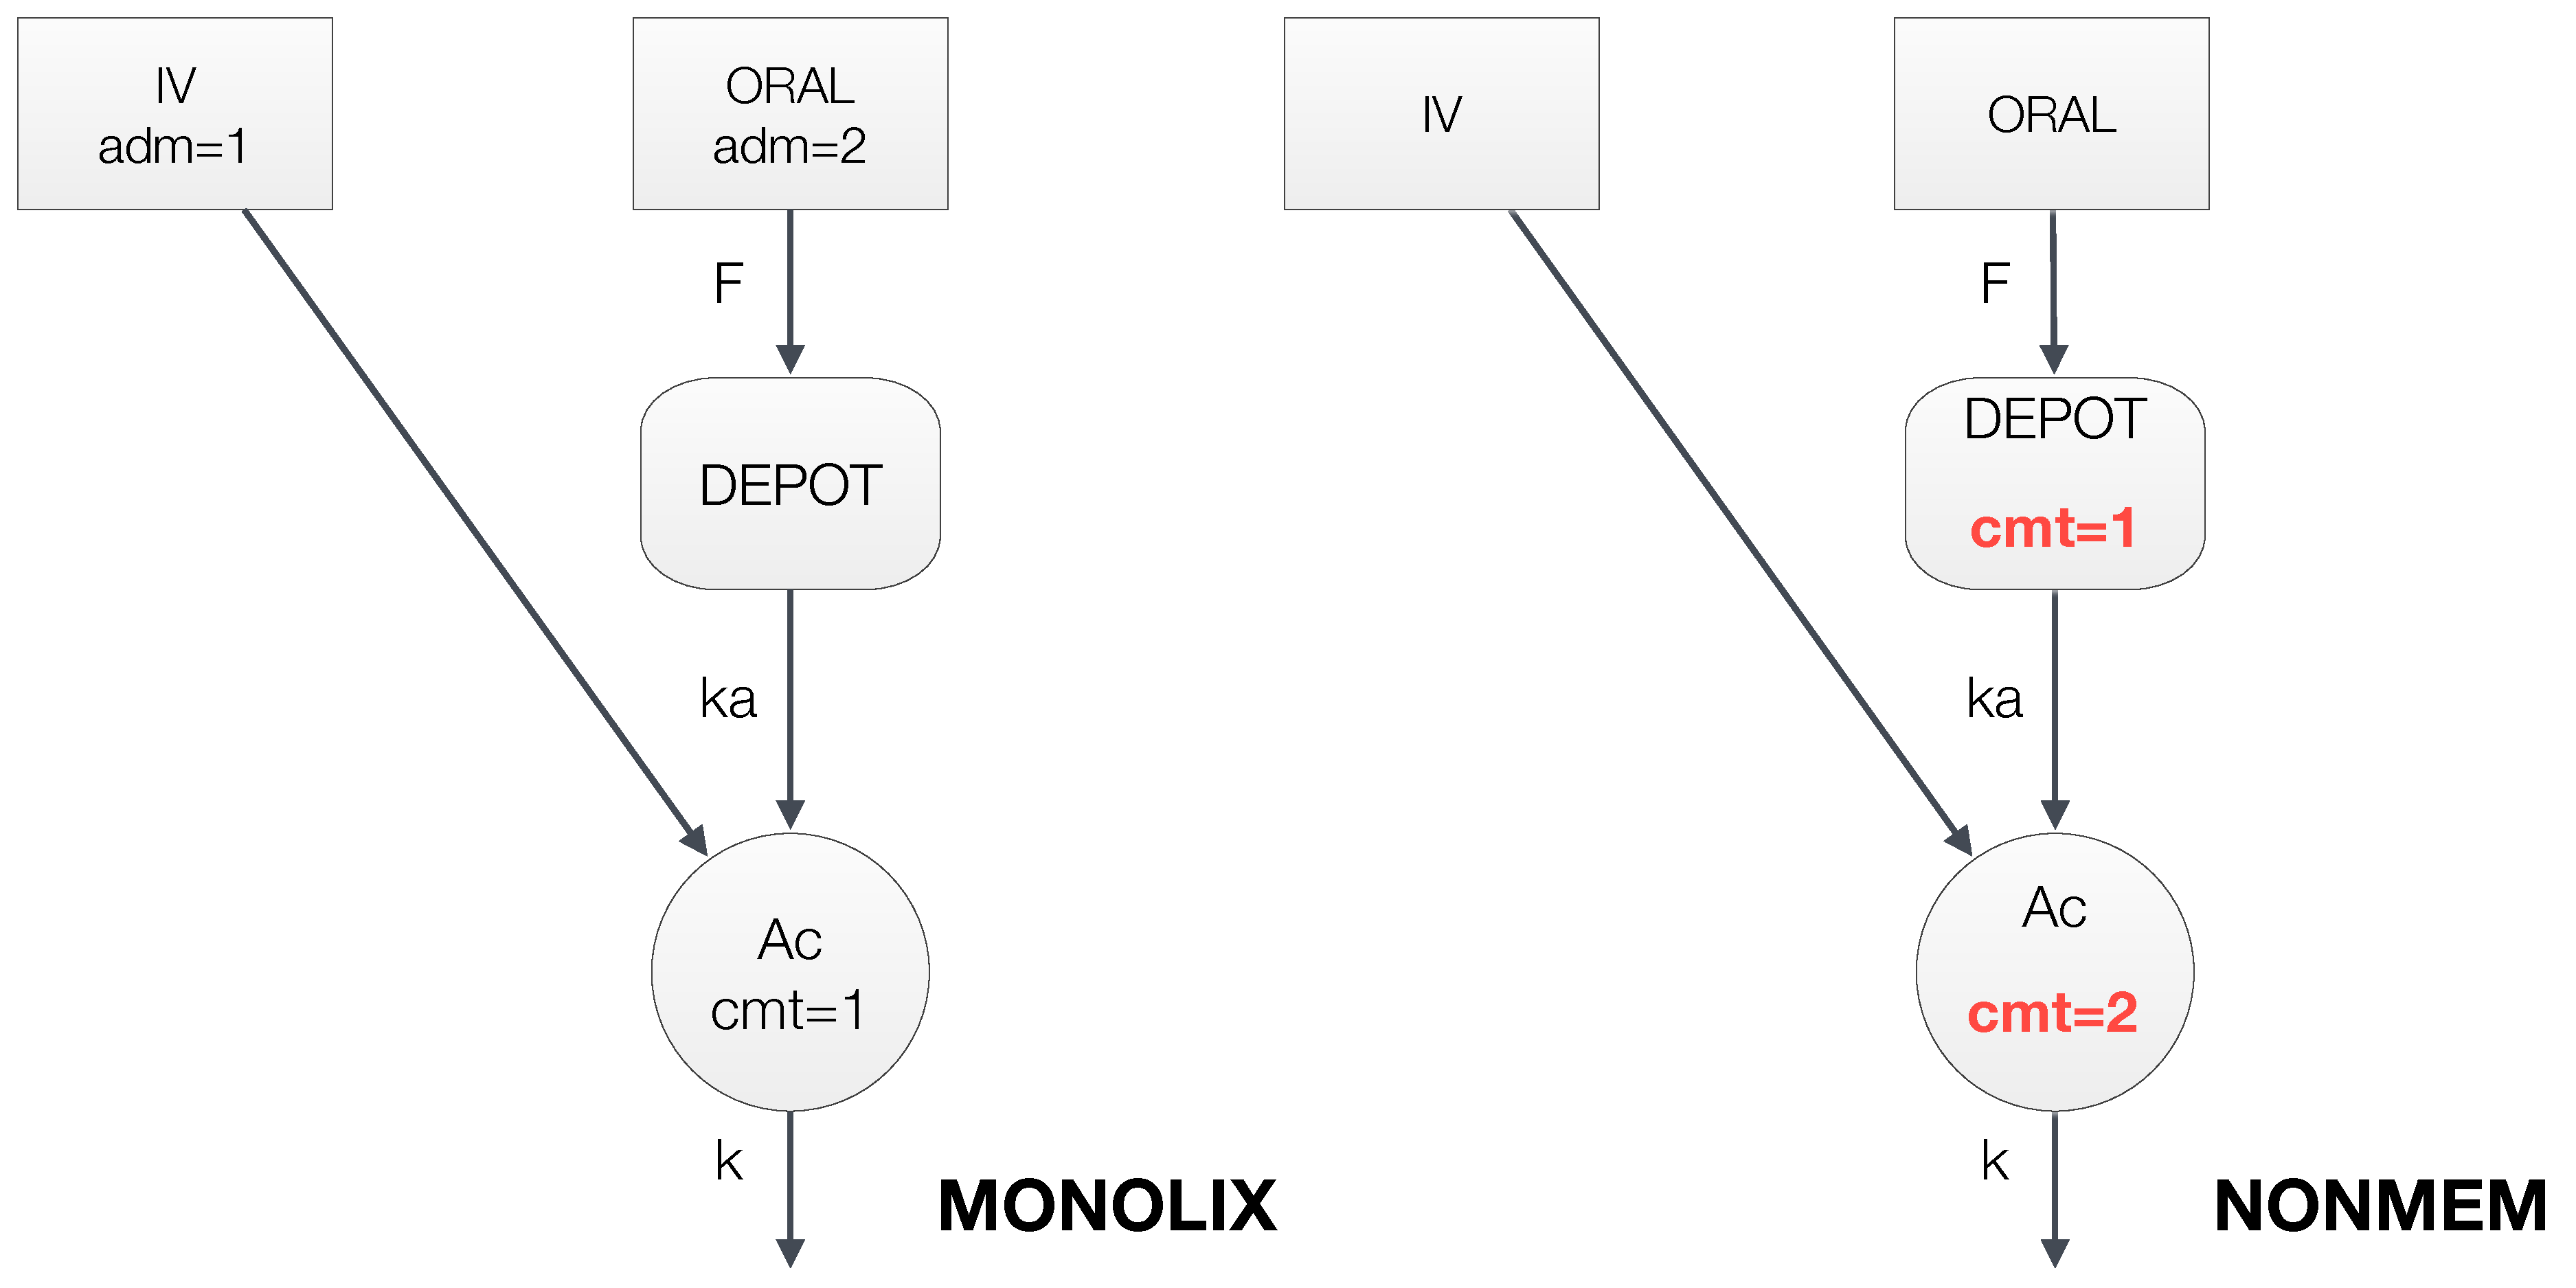
\includegraphics[width=130mm]{pics/ComplexModel1b}
\caption{C1b model, with compartment numbering dependent on the target tool.}
\label{fig:ComplexModel1b}
\end{figure}

\begin{table}[ht!]
\footnotesize
\parbox{.5\linewidth}{
\centering
\begin{tabular}{ccccc}
  \hline
     \multicolumn{5}{c}{\textbf{MONOLIX}} \\
  \hline
ID	& TIME  & AMT	 & \textbf{ADM} &	Y \\
  \hline
1	& 0	    & 2.24	& \textbf{1}	& . \\
1	& 1	    & .	& .		 	& 142 \\
1	& 2	    & .	& .	 		& 54.9 \\
...     &  ...     &  ...     & ...  			& ...\\
1	& 6	    & 7	& \textbf{2}	& . \\
1	& 7	    & .	& .			& 192 \\
1	& 8	    & .	& .			& 141 \\
...     &  ...     &  ...     & ...  			& ...\\
2	& 0	    & 2.73	& \textbf{1}	& . \\
2	& 1	    & . 	& .			& 176 \\
...     &  ...     &  ...     & ...  			& ...\\
\end{tabular}
}
\hfill
\parbox{.5\linewidth}{
\centering
\begin{tabular}{ccccc}
  \hline
   \multicolumn{5}{c}{\textbf{NONMEM}} \\
  \hline
ID	& TIME  & AMT	 & \textbf{\textcolor{red}{CMT}} &	DV \\
  \hline
1	& 0	    & 2.24	& \textbf{\textcolor{red}{2}}	& . \\
1	& 1	    & .	& 2		 	& 142 \\
1	& 2	    & .	& 2	 		& 54.9 \\
...     &  ...     &  ...     & ...  			& ...\\
1	& 6	    & 7	& \textbf{\textcolor{red}{1}}	& . \\
1	& 7	    & .	& 2			& 192 \\
1	& 8	    & .	& 2			& 141 \\
...     &  ...     &  ...     & ...  			& ...\\
2	& 0	    & 2.73	& \textbf{\textcolor{red}{2}}	& . \\
2	& 1	    & . 	& 2	 		& 176 \\
...     &  ...     &  ...     & ...  			& ...\\
\end{tabular}
}
\caption{NONMEM and MONOLIX datasets for the C1b model. In contrast to the previous case, a 
renumbering is required when transforming the data and renaming the ADM to CMT column.}
\label{tab:C1bTable}
\end{table}

\begin{table}[h!]
\setlength{\tabcolsep}{15pt}
\begin{center}
\begin{tabular}{c}
%\begin{tabular*}{.95\textwidth}{@{\extracolsep{\fill} } ll}
  \hline \hline
PK macro  \\[-.25ex]
  \hline
\lstset{language=NONMEMdataSet}
\begin{lstlisting}
input = {F, ka, V, k}
PK:
compartment(cmt=1, amount=Ac)
oral(adm=[*2*], cmt=1, ka, p=F)
iv(adm=[*1*], cmt=1)
elimination(cmt=1, k)
Cc = Ac/V
\end{lstlisting}
%&
%\lstset{language=NONMEMdataSet}
%\begin{lstlisting}
%input = {F, ka, V, k}
%PK:
%compartment(cmt=1, amount=Ac)
%[*compartment(cmt=2, amount=Depot)*]
%oral(adm=1, [*fromCmt=2,*] cmt=1, ka, p=F)
%iv(adm=2, cmt=1)
%elimination(cmt=1, k)
%Cc = Ac/V
%\end{lstlisting} 
\\
  \hline
\end{tabular}
\caption{PK macros  for the C1b model, as shown in Figure \ref{fig:ComplexModel1b} (left).}
\label{tab:C1bMacrosTable}
\end{center}
\end{table}


PharmML code is identical to the previous example, and will not be shown, except the 
amended \xatt{adm} attribute assignments, \xatt{adm=\textbf{\textcolor{red}{2}}} for oral 
and \xatt{adm=\textbf{\textcolor{red}{1}}} for IV administration, see Table \ref{tab:C1bMacrosTable}.
%\lstset{language=XML}
%\begin{lstlisting}
%                <Oral>
%                    <Value argument="adm">
%                        <ct:Int>2</ct:Int>
%                    </Value>
%                    <!-- omitted details -->
%                </Oral>
%                
%                <IV>
%                    <Value argument="adm">
%                        <ct:Int>1</ct:Int>
%                    </Value>
%                    <!-- omitted details -->
%                </IV>
%\end{lstlisting}


%\cleardoublepage
%%%%%%%%%%%%%%%%%%%%%%%%%%%%%%%%%%%%%%%%%%%%%%%%%%%%%%%
\subsection{Example C2}
Modified from \cite{MLXTRANforMonolix:2014}. This model can be modelled by the 
ADVAN12 routine, with an additional IV administration.

\begin{figure}[htbp]
\centering
 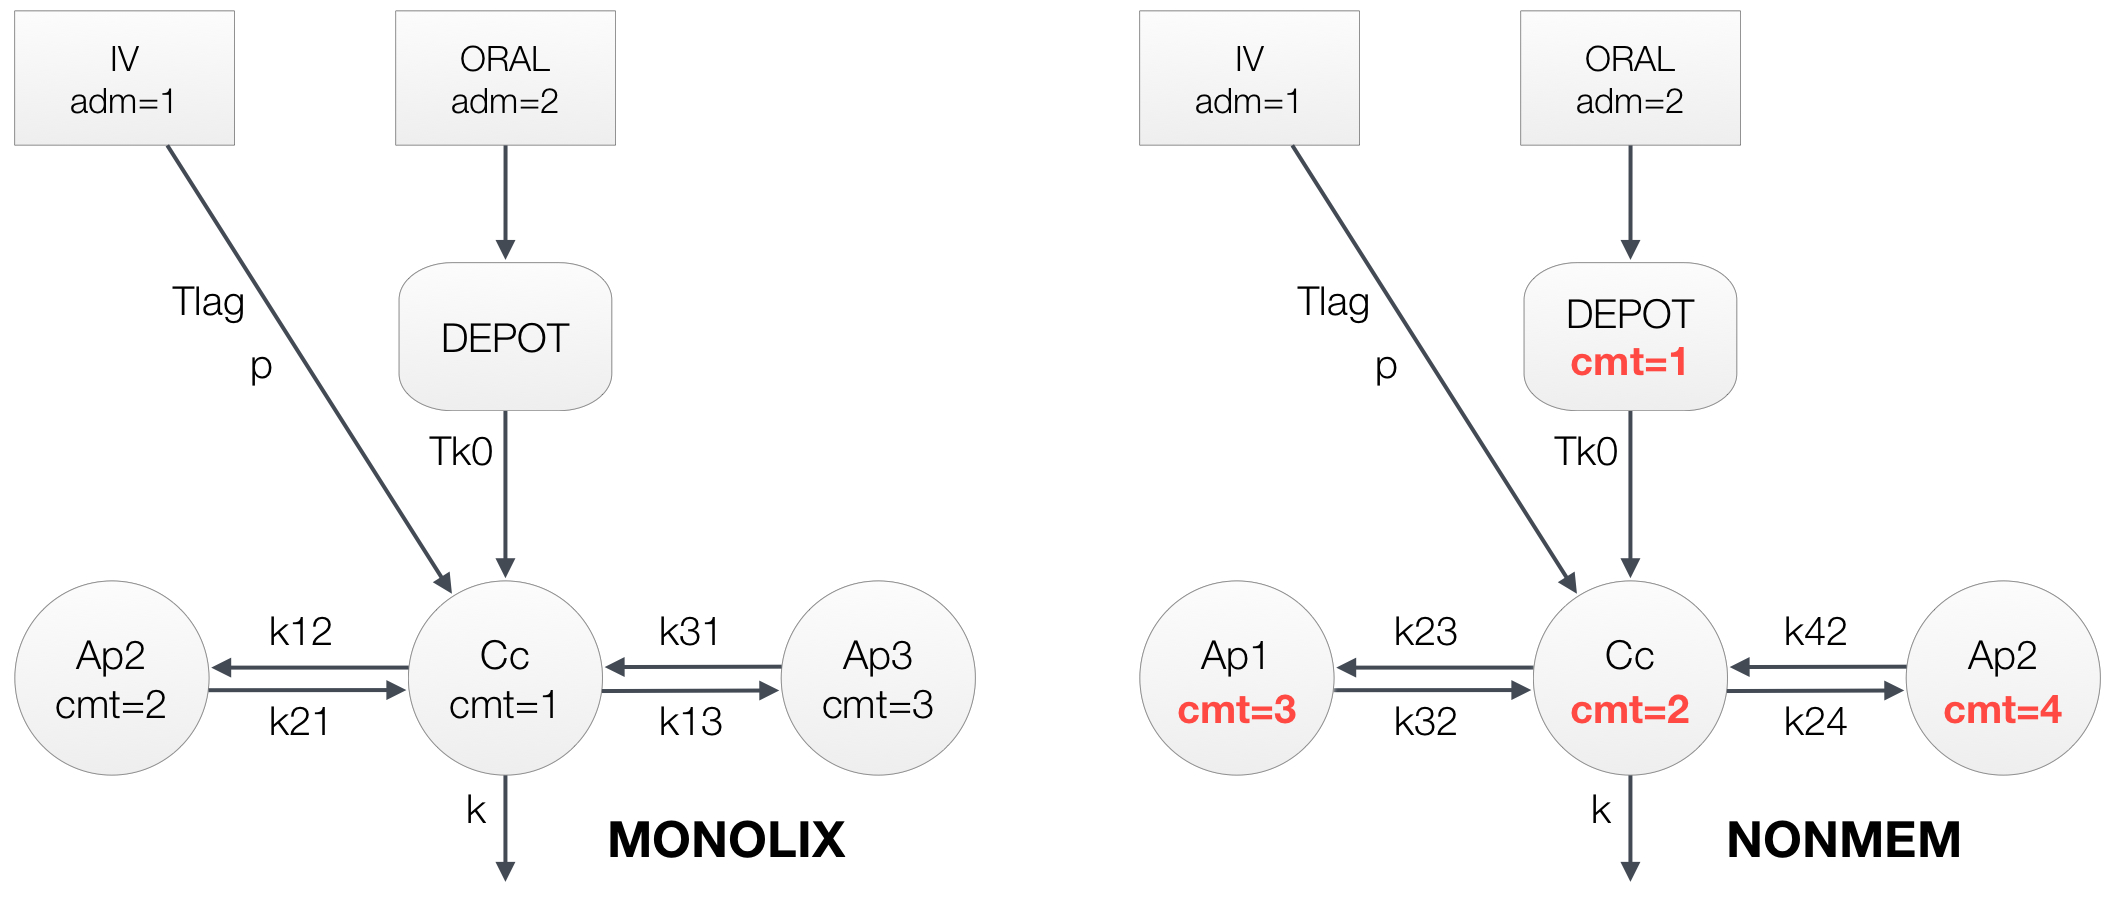
\includegraphics[width=160mm]{pics/ComplexModel2}
\caption{C2 model, with compartment numbering dependent on the target tool.}
\label{fig:ComplexModel2}
\end{figure}


\begin{table}[h!]
\footnotesize
\parbox{.5\linewidth}{
\centering
\begin{tabular}{cccccc}
  \hline
   \multicolumn{6}{c}{\textbf{MONOLIX}} \\
  \hline
ID	& TIME  & AMT	 & \textbf{ADM} &  TINF &	Y \\
  \hline
1	& 6	    & 10	& \textbf{1}	 & 2	 & . \\
1	& 9	    & 20	& \textbf{2}	 & .	 & . \\
1	& 18	    & 10	& \textbf{1}	 & 2	 & . \\
1	& 30	    & 10	& \textbf{1}	 & 2	 & . \\
1	& 33	    & 20	& \textbf{2}	 & .	 & . \\
...     &  ...     &  ...     &  ...  & ...  & ... \\
1	& 0	    & .	& .	& .	& 0 \\
1	& 6	    & .	& .	& .	& 0 \\
1	& 12	    & .	& .	& .	& 1.18 \\
...     &  ...     &  ...     & ...  & ...  & ...\\
\end{tabular}
}
\hfill
\parbox{.5\linewidth}{
\centering
\begin{tabular}{cccccc}
  \hline
   \multicolumn{6}{c}{\textbf{NONMEM}} \\
  \hline
ID	& TIME  & AMT	 & \textbf{\textcolor{red}{CMT}} &  RATE &	DV \\
  \hline
1	& 6	    & 10	& \textbf{\textcolor{red}{1}}	 & 5	 & . \\
1	& 9	    & 20	& \textbf{\textcolor{red}{2}}	 & .	 & . \\
1	& 18	    & 10	& \textbf{\textcolor{red}{1}}	 & 5	 & . \\
1	& 30	    & 10	& \textbf{\textcolor{red}{1}}	 & 5	 & . \\
1	& 33	    & 20	& \textbf{\textcolor{red}{2}}	 & .	 & . \\
...     &  ...     &  ...     &  ...  & ...  & ... \\
1	& 0	    & .	& 1	& .	& 0 \\
1	& 6	    & .	& 1	& .	& 0 \\
1	& 12	    & .	& 1	& .	& 1.18 \\
...     &  ...     &  ...     & ...  & ...  & ...\\
\end{tabular}
}
\caption{NONMEM and MONOLIX datasets for the C2 model.}
\end{table}


\begin{table}[ht!]
\setlength{\tabcolsep}{1pt}
\begin{center}
\begin{tabular}{c}
%\begin{tabular*}{1.05\textwidth}{@{\extracolsep{\fill} } ll}
  \hline \hline
PK macro  \\[-.25ex]
  \hline
\lstset{language=NONMEMdataSet}
\begin{lstlisting}
input = {V, alpha, beta} 
PK:
compartment(cmt=1, volume=V, concentration=Cc)
iv(adm=1, cmt=1, p=0.1, Tlag=t/(t + 10))
oral(adm=2, cmt=1, Tk0=0.1)
elimination(cmt=1, k=0.2)
peripheral(k12=0.6, k21=0.8, amount=Ap2)
peripheral(k13=0.6+alpha, k31=0.8+beta, amount=Ap3)
\end{lstlisting}
%&
%\lstset{language=NONMEMdataSet}
%\begin{lstlisting}
%compartment(cmt=1, volume=V, concentration=Cc)
%[*compartment(cmt=4, amount=Depot1)*]
%iv(adm=1, cmt=1, p=0.1, Tlag=t/(t + 10))
%oral(adm=2, [*fromCmt=4,*] cmt=1, Tk0=0.1)
%elimination(cmt=1, k=0.2)
%peripheral(k12=0.6, k21=0.8, amount=Ap2)
%peripheral(k13=0.6+alpha, k31=0.8+beta, amount=Ap3)
%\end{lstlisting} 
\\
  \hline
\end{tabular}
\caption{PK macros  for the C2 model, as shown in Figure \ref{fig:ComplexModel2} (left).}
\label{tab:C3Table}
\end{center}
\end{table}


PharmML code:
\lstset{language=XML}
\begin{lstlisting}
        <StructuralModel blkId="smC2">
            <ct:Variable symbolType="real" symbId="Ap2"/>
            <ct:Variable symbolType="real" symbId="Ap3"/>
            <ct:Variable symbolType="real" symbId="Cc"/>
            
            <PKmacros>
                <Compartment>
                    <Value argument="cmt">
                        <ct:Int>1</ct:Int>
                    </Value>
                    <Value argument="volume">
                        <ct:SymbRef blkIdRef="pm1" symbIdRef="V"/>
                    </Value>
                    <Value argument="concentration">
                        <ct:SymbRef symbIdRef="Cc"/>
                    </Value>
                </Compartment>
                
                <IV>
                    <Value argument="adm">
                        <ct:Int>1</ct:Int>
                    </Value>
                    <Value argument="cmt">
                        <ct:Int>1</ct:Int>
                    </Value>
                    <Value argument="p">
                        <ct:Real>0.1</ct:Real>
                    </Value>
                    <Value argument="Tlag">
                        <ct:Assign>
                            <math:Equation>
                                <math:Binop op="divide">
                                    <ct:SymbRef symbIdRef="t"/>
                                    <math:Binop op="plus">
                                        <ct:SymbRef symbIdRef="t"/>
                                        <ct:Real>10</ct:Real>
                                    </math:Binop>
                                </math:Binop>
                            </math:Equation>
                        </ct:Assign>
                    </Value>
                </IV>
                
                <Oral>
                    <Value argument="adm">
                        <ct:Int>2</ct:Int>
                    </Value>
                    <Value argument="cmt">
                        <ct:Int>1</ct:Int>
                    </Value>
                    <Value argument="Tk0">
                        <ct:Real>0.1</ct:Real>
                    </Value>
                </Oral>
                
                <Elimination>
                    <Value argument="cmt">
                        <ct:Int>1</ct:Int>
                    </Value>
                    <Value argument="k">
                        <ct:Real>0.2</ct:Real>
                    </Value>
                </Elimination>
                
                <Peripheral>
                    <Value argument="k12">
                        <ct:Real>0.6</ct:Real>
                    </Value>
                    <Value argument="k21">
                        <ct:Real>0.8</ct:Real>
                    </Value>
                    <Value argument="amount">
                        <ct:SymbRef symbIdRef="Ap2"/>
                    </Value>
                </Peripheral>
                
                <Peripheral>
                    <Value argument="k13">
                        <ct:Assign>
                            <math:Equation>
                                <math:Binop op="plus">
                                    <ct:Real>0.6</ct:Real>
                                    <ct:SymbRef blkIdRef="pm1" symbIdRef="alpha"/>
                                </math:Binop>
                            </math:Equation>
                        </ct:Assign>
                    </Value>
                    <Value argument="k31">
                        <ct:Assign>
                            <math:Equation>
                                <math:Binop op="plus">
                                    <ct:Real>0.8</ct:Real>
                                    <ct:SymbRef blkIdRef="pm1" symbIdRef="beta"/>
                                </math:Binop>
                            </math:Equation>
                        </ct:Assign>
                    </Value>
                    <Value argument="amount">
                        <ct:SymbRef symbIdRef="Ap3"/>
                    </Value>
                </Peripheral>
                
            </PKmacros>
        </StructuralModel>
\end{lstlisting}



%\cleardoublepage
%%%%%%%%%%%%%%%%%%%%%%%%%%%%%%%%%%%%%%%%%%%%%%%%%%%%%%%
\subsection{Example C3}
From \cite{MLXTRANforMonolix:2014}. Figure \ref{fig:ComplexModel3} is illustrating this model in two versions. 

\begin{figure}[htbp]
\centering
 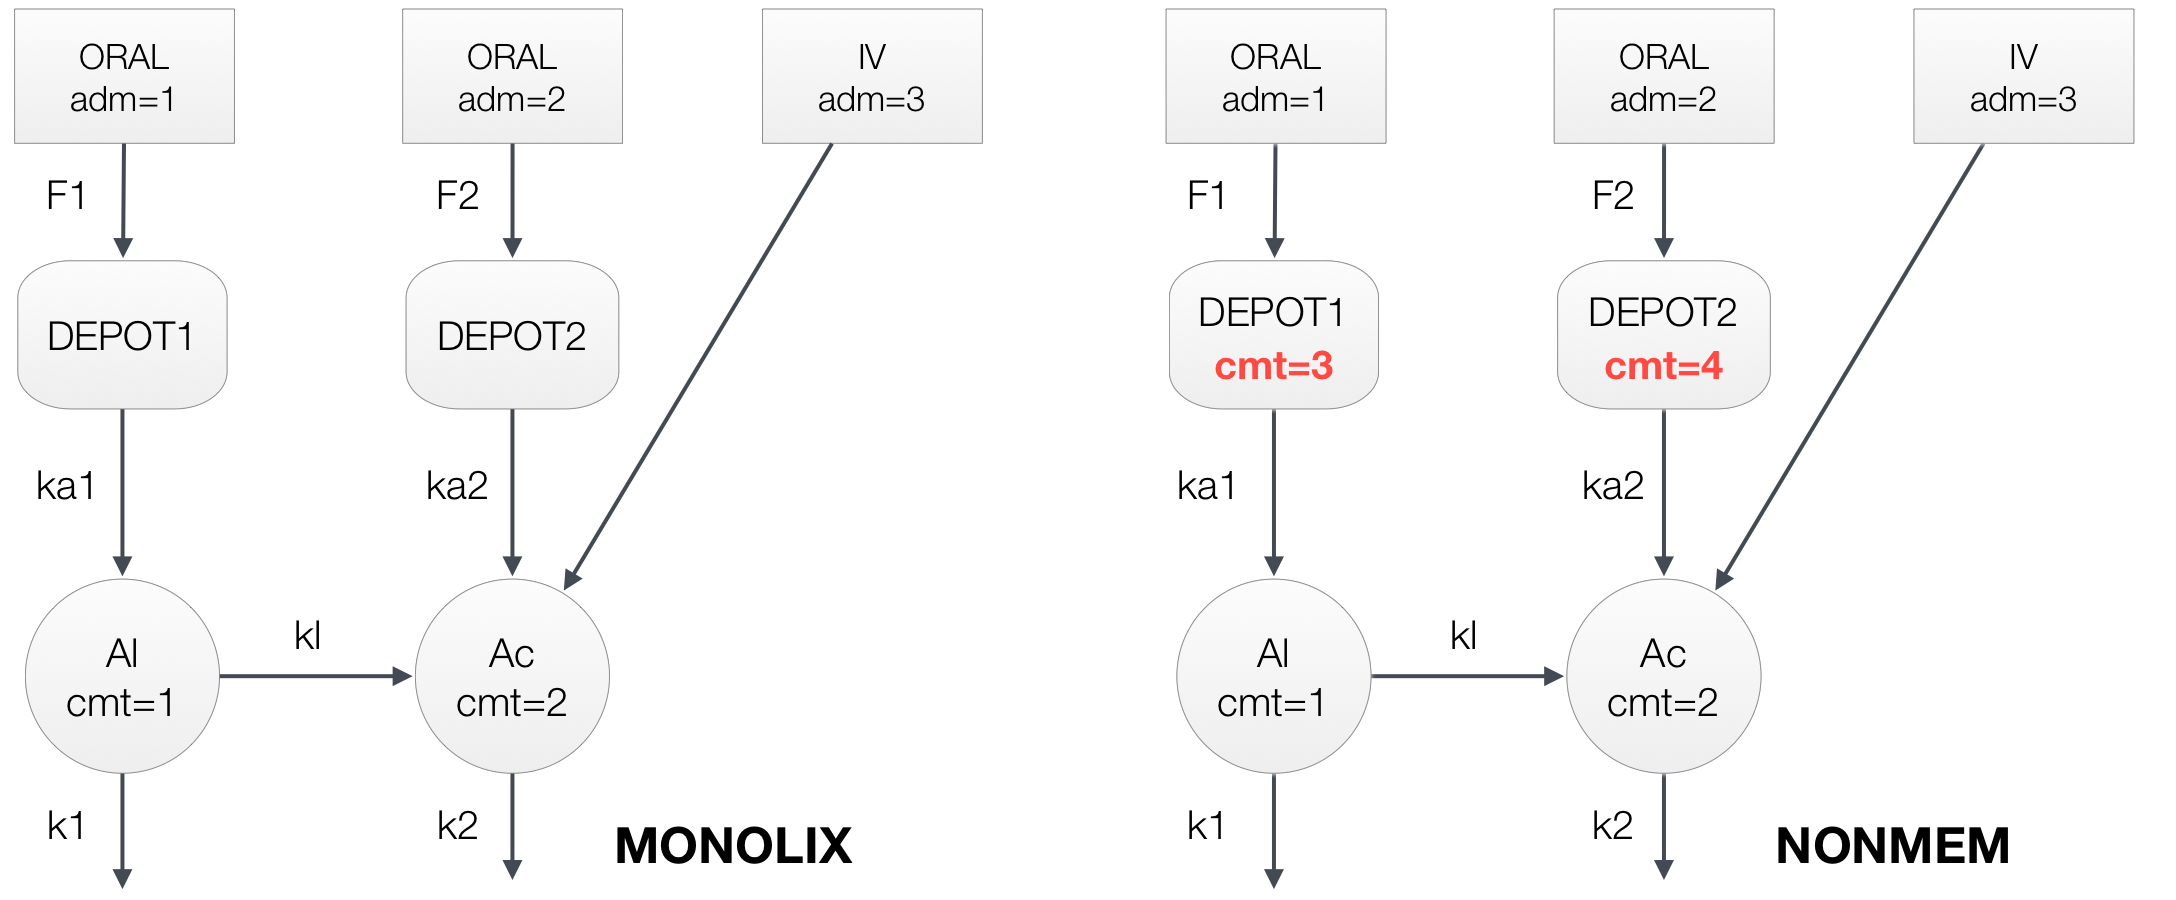
\includegraphics[width=160mm]{pics/ComplexModel3}
\caption{C3 model, with compartment numbering dependent on the target tool.}
\label{fig:ComplexModel3}
\end{figure}

\begin{table}[h!]
\footnotesize
\parbox{.5\linewidth}{
\centering
\begin{tabular}{cccccc}
  \hline
   \multicolumn{6}{c}{\textbf{MONOLIX}} \\
  \hline
ID	& TIME  & AMT	 & \textbf{ADM} &  TINF &	Y \\
  \hline
1	& 6	    & 10	& \textbf{1}	 & .	 & . \\
1	& 9	    & 20	& \textbf{2}	 & .	 & . \\
1	& 12	    & 30	& \textbf{3}	 & 2	 & . \\
1	& 18	    & 10	& \textbf{1}	 & .	 & . \\
1	& 30	    & 10	& \textbf{1}	 & .	 & . \\
1	& 33	    & 20	& \textbf{2}	 & .	 & . \\
1	& 36	    & 30	& \textbf{3}	 & 2	 & . \\
...     &  ...     &  ...     &  ...  & ...  & ... \\
1	& 0	    & .	& .	& .	& 0 \\
1	& 6	    & .	& .	& .	& 0 \\
1	& 12	    & .	& .	& .	& 1.18 \\
...     &  ...     &  ...     & ...  & ...  & ...\\
\end{tabular}
}
\hfill
\parbox{.5\linewidth}{
\centering
\begin{tabular}{cccccc}
  \hline
   \multicolumn{6}{c}{\textbf{NONMEM}} \\
  \hline
ID	& TIME  & AMT	 & \textbf{\textcolor{red}{CMT}} &  RATE &	DV \\
  \hline
1	& 6	    & 10	& \textbf{\textcolor{red}{3}}	 & .	 & . \\
1	& 9	    & 20	& \textbf{\textcolor{red}{4}}	 & .	 & . \\
1	& 12	    & 30	& \textbf{\textcolor{red}{2}}	 & \textbf{15}	 & . \\
1	& 18	    & 10	& \textbf{\textcolor{red}{3}}	 & .	 & . \\
1	& 30	    & 10	& \textbf{\textcolor{red}{3}}	 & .	 & . \\
1	& 33	    & 20	& \textbf{\textcolor{red}{4}}	 & .	 & . \\
1	& 36	    & 30	& \textbf{\textcolor{red}{2}}	 & \textbf{15}	 & . \\
...     &  ...     &  ...     &  ...  & ...  & ... \\
1	& 0	    & .	& 1	& .	& 0 \\
1	& 6	    & .	& 1	& .	& 0 \\
1	& 12	    & .	& 1	& .	& 1.18 \\
...     &  ...     &  ...     & ...  & ...  & ...\\
\end{tabular}
}
\caption{NONMEM and MONOLIX datasets for the C3 model.}
\end{table}

\begin{table}[ht!]
\setlength{\tabcolsep}{15pt}
\begin{center}
\begin{tabular}{c}
%\begin{tabular*}{.95\textwidth}{@{\extracolsep{\fill} } ll}
  \hline \hline
PK macro  \\[-.25ex]
  \hline
\lstset{language=NONMEMdataSet}
\begin{lstlisting}
input = {F1, F2, ka1, ka2, k1, k2, kl, V}
PK:
compartment(cmt=1, amount=Al)
compartment(cmt=2, amount=Ac, volume=V)
oral(adm=1, cmt=1, ka1, p=F1)
oral(adm=2, cmt=2, ka2, p=F2)
iv(adm=3, cmt=2)
transfer(from=1, to=2, kt=kl)
elimination(cmt=1, k1)
elimination(cmt=2, k2)
\end{lstlisting}
%&
%\lstset{language=NONMEMdataSet}
%\begin{lstlisting}
%input = {F1, F2, ka1, ka2, k1, k2, kl, V}
%PK:
%compartment(cmt=1, amount=Al)                                                   
%compartment(cmt=2, amount=Ac)
%[*compartment(cmt=3, amount=Depot1)*]
%[*compartment(cmt=4, amount=Depot2)*]
%oral(adm=1, [*fromCmt=3,*] cmt=1, ka1, p=F1)
%oral(adm=2, [*fromCmt=4,*] cmt=2, ka2, p=F2)
%iv(adm=3, cmt=2)
%transfer(from=1, to=2, kt=kl)
%elimination(cmt=1, k1)
%elimination(cmt=2, k2)
%Cc = Ac/V
%\end{lstlisting} 
\\
  \hline
\end{tabular}
\caption{PK macros  for the C3 model, as shown in Figure \ref{fig:ComplexModel3} (left).}
\label{tab:C2Table}
\end{center}
\end{table}


PharmML code:
\lstset{language=XML}
\begin{lstlisting}
        <StructuralModel blkId="smC3">
            <ct:Variable symbolType="real" symbId="Al"/>
            <ct:Variable symbolType="real" symbId="Ac"/>
            <ct:Variable symbolType="real" symbId="Cc"/>
            
            <PKmacros>
                <Compartment>
                    <Value argument="cmt">
                        <ct:Int>1</ct:Int>
                    </Value>
                    <Value argument="amount">
                        <ct:SymbRef symbIdRef="Al"/>
                    </Value>
                </Compartment>
                
                <Compartment>
                    <Value argument="cmt">
                        <ct:Int>2</ct:Int>
                    </Value>
                    <Value argument="amount">
                        <ct:SymbRef symbIdRef="Ac"/>
                    </Value>
                    <Value argument="volume">
                        <ct:SymbRef blkIdRef="pm1" symbIdRef="V"/>
                    </Value>
                </Compartment>
                
                <Oral>
                    <Value argument="adm">
                        <ct:Int>1</ct:Int>
                    </Value>
                    <Value argument="cmt">
                        <ct:Int>1</ct:Int>
                    </Value>
                    <Value>
                        <ct:SymbRef blkIdRef="pm1" symbIdRef="ka1"/>
                    </Value>
                    <Value argument="p">
                        <ct:SymbRef blkIdRef="pm1" symbIdRef="F1"/>
                    </Value>
                </Oral>
                
                <Oral>
                    <Value argument="adm">
                        <ct:Int>2</ct:Int>
                    </Value>
                    <Value argument="cmt">
                        <ct:Int>2</ct:Int>
                    </Value>
                    <Value>
                        <ct:SymbRef blkIdRef="pm1" symbIdRef="ka2"/>
                    </Value>
                    <Value argument="p">
                        <ct:SymbRef blkIdRef="pm1" symbIdRef="F2"/>
                    </Value>
                </Oral>
                
                <IV>
                    <Value argument="adm">
                        <ct:Int>3</ct:Int>
                    </Value>
                    <Value argument="cmt">
                        <ct:Int>2</ct:Int>
                    </Value>
                </IV>
                
                <Transfer>
                    <Value argument="from">
                        <ct:Int>1</ct:Int>
                    </Value>
                    <Value argument="to">
                        <ct:Int>2</ct:Int>
                    </Value>
                    <Value argument="kt">
                        <ct:SymbRef blkIdRef="pm1" symbIdRef="kl"/>
                    </Value>
                </Transfer>
                
                <Elimination>
                    <Value argument="cmt">
                        <ct:Int>1</ct:Int>
                    </Value>
                    <Value>
                        <ct:SymbRef blkIdRef="pm1" symbIdRef="k1"/>
                    </Value>
                </Elimination>
                
                <Elimination>
                    <Value argument="cmt">
                        <ct:Int>1</ct:Int>
                    </Value>
                    <Value>
                        <ct:SymbRef blkIdRef="pm1" symbIdRef="k2"/>
                    </Value>
                </Elimination>
                
            </PKmacros>
        </StructuralModel>
\end{lstlisting}


%\cleardoublepage
%%%%%%%%%%%%%%%%%%%%%%%%%%%%%%%%%%%%%%%%%%%%%%%%%%%%%%%
\subsection{Example C4}
The following example is from 'Four models' document \cite{LavielleFourModels:2014}.
%Here the original description:
%"In this example, one type of dose is administered orally (adm=1) and absorbed into a latent 
%compartment following a first-order absorption process, a second type is administered o
%rally (adm=2) and absorbed into the central compartment following a zero-order absorption process,
%a third type is directly administered intravenously to the central compartment (adm=3).
%The transfer from the latent to the central compartment is linear. A peripheral compartment
%is linked to the central compartment. The drug is eliminated by a linear process from the
%latent compartment and a nonlinear process from the central one. Here, Al and Ac are the
%drug amounts in the latent and central compartments." 
Figure \ref{fig:ComplexModel4} is illustrating this model in two versions. 

\begin{figure}[htbp!]
\centering
 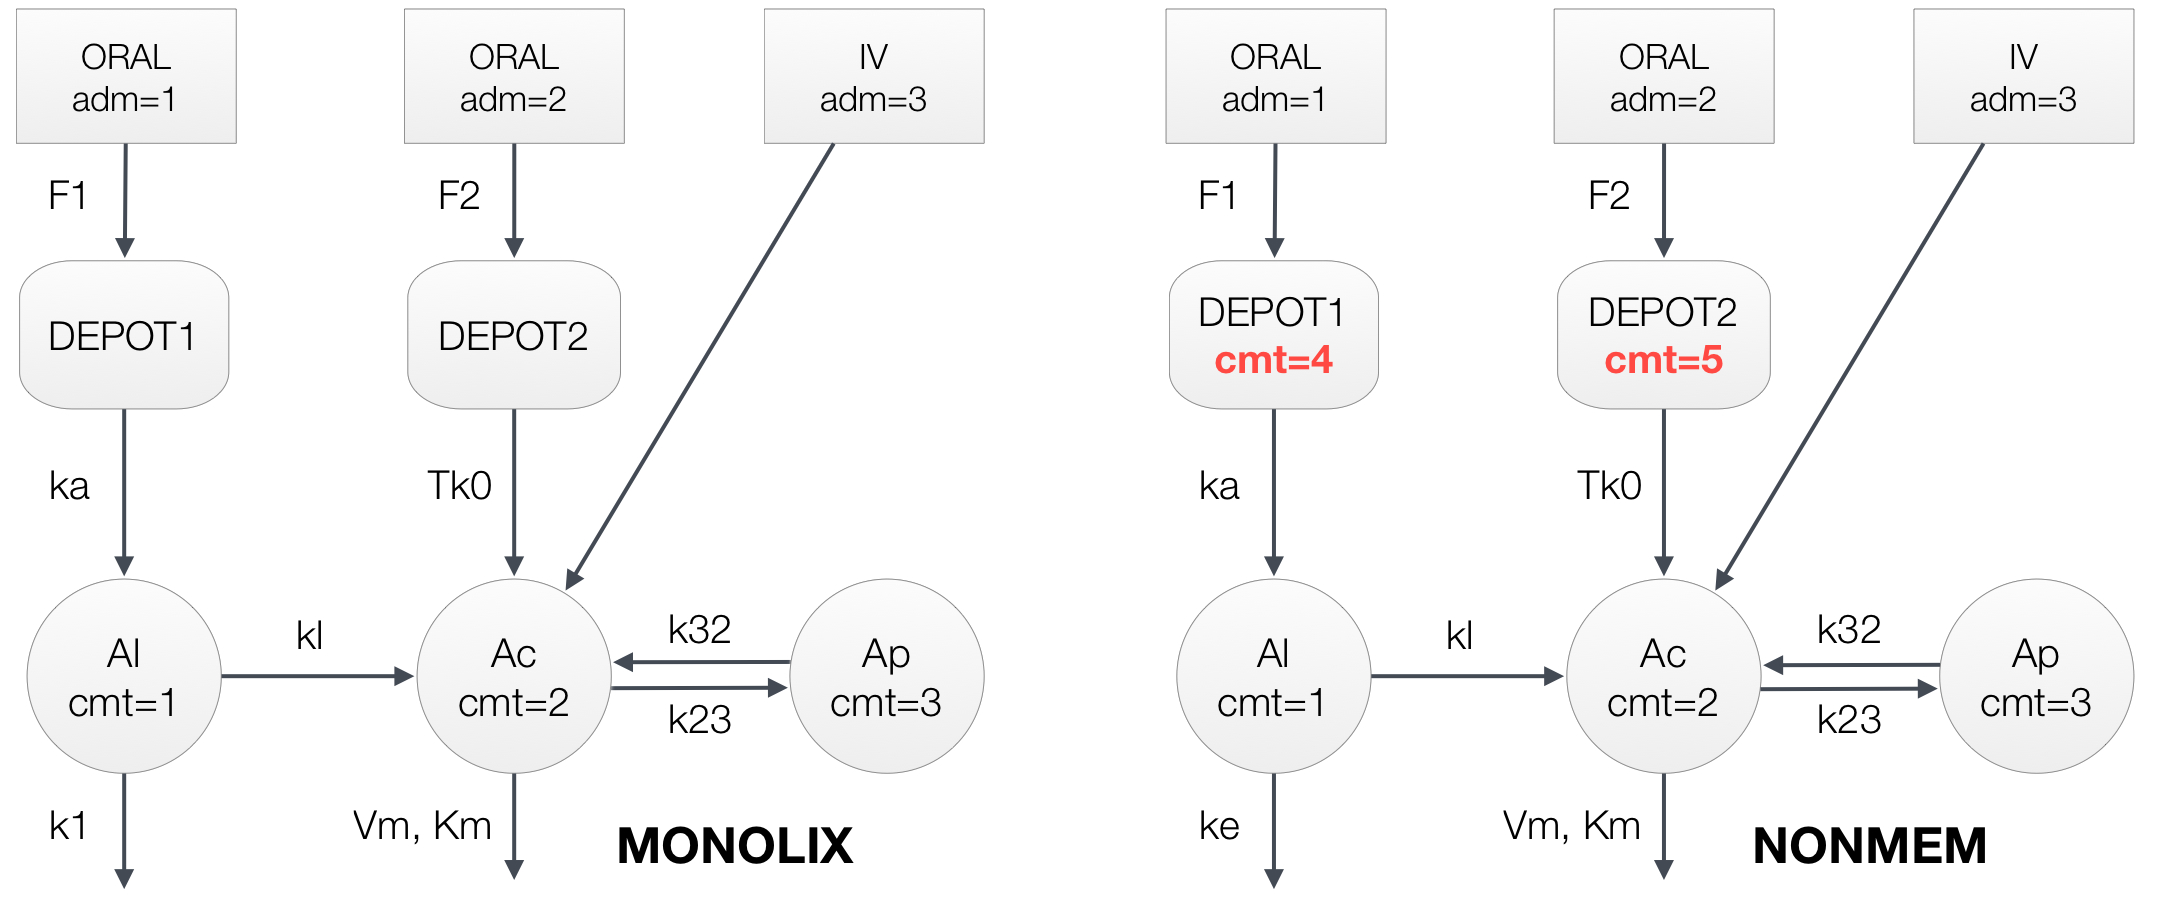
\includegraphics[width=160mm]{pics/ComplexModel4}
\caption{C4 model, with compartment numbering dependent on the target tool.}
\label{fig:ComplexModel4}
\end{figure}

\begin{table}[h!]
\footnotesize
\parbox{.5\linewidth}{
\centering
\begin{tabular}{cccccc}
  \hline
   \multicolumn{6}{c}{\textbf{MONOLIX}} \\
  \hline
ID	& TIME  & AMT	 & \textbf{ADM} &  TINF &	Y \\
  \hline
1	& 6	    & 10	& \textbf{1}	 & .	 & . \\
1	& 9	    & 20	& \textbf{2}	 & .	 & . \\
1	& 12	    & 30	& \textbf{3}	 & 2	 & . \\
1	& 18	    & 10	& \textbf{1}	 & .	 & . \\
1	& 30	    & 10	& \textbf{1}	 & .	 & . \\
1	& 33	    & 20	& \textbf{2}	 & .	 & . \\
1	& 36	    & 30	& \textbf{3}	 & 2	 & . \\
...     &  ...     &  ...     &  ...  & ...  & ... \\
1	& 0	    & .	& .	& .	& 0 \\
1	& 6	    & .	& .	& .	& 0 \\
1	& 12	    & .	& .	& .	& 1.18 \\
...     &  ...     &  ...     & ...  & ...  & ...\\
\end{tabular}
}
\hfill
\parbox{.5\linewidth}{
\centering
\begin{tabular}{cccccc}
  \hline
   \multicolumn{6}{c}{\textbf{NONMEM}} \\
  \hline
ID	& TIME  & AMT	 & \textbf{\textcolor{red}{CMT}} &  RATE &	DV \\
  \hline
1	& 6	    & 10	& \textbf{\textcolor{red}{4}}	 & .	 & . \\
1	& 9	    & 20	& \textbf{\textcolor{red}{5}}	 & .	 & . \\
1	& 12	    & 30	& \textbf{\textcolor{red}{2}}	 & \textbf{15}	 & . \\
1	& 18	    & 10	& \textbf{\textcolor{red}{4}}	 & .	 & . \\
1	& 30	    & 10	& \textbf{\textcolor{red}{4}}	 & .	 & . \\
1	& 33	    & 20	& \textbf{\textcolor{red}{5}}	 & .	 & . \\
1	& 36	    & 30	& \textbf{\textcolor{red}{2}}	 & \textbf{15}	 & . \\
...     &  ...     &  ...     &  ...  & ...  & ... \\
1	& 0	    & .	& 1	& .	& 0 \\
1	& 6	    & .	& 1	& .	& 0 \\
1	& 12	    & .	& 1	& .	& 1.18 \\
...     &  ...     &  ...     & ...  & ...  & ...\\
\end{tabular}
}
\caption{NONMEM and MONOLIX datasets for the C4 model.}
\end{table}

\begin{table}[ht!]
\setlength{\tabcolsep}{15pt}
\begin{center}
\begin{tabular}{c}
%\begin{tabular*}{.95\textwidth}{@{\extracolsep{\fill} } ll}
  \hline \hline
PK macro  \\[-.25ex]
  \hline
\lstset{language=NONMEMdataSet}
\begin{lstlisting}
input = {F1, F2, ka, Tk0, kl, V, k, Vm, Km}
PK:
compartment(cmt=1, amount=Al)
compartment(cmt=2, amount=Ac)
oral(adm=1, cmt=1, ka, p=F1)
oral(adm=2, cmt=2, Tk0, p=F2)
iv(adm=3, cmt=2)
transfer(from=1, to=2, kt=kl)
peripheral(k23, k32, amount=Ap)
elimination(cmt=1, k)
elimination(cmt=2, Km, Vm)
\end{lstlisting}
\\
  \hline
\end{tabular}
\caption{PK macros  for the C4 model, as shown in Figure \ref{fig:ComplexModel4} (left).}
\label{tab:C4Table}
\end{center}
\end{table}


PharmML code:
\lstset{language=XML}
\begin{lstlisting}
        <StructuralModel blkId="smC4">
            <ct:Variable symbolType="real" symbId="Al"/>
            <ct:Variable symbolType="real" symbId="Ac"/>
            <ct:Variable symbolType="real" symbId="Cc">
                <ct:Assign>
                    <math:Equation>
                        <math:Binop op="divide">
                            <ct:SymbRef symbIdRef="Ac"/>
                            <ct:SymbRef blkIdRef="pm1" symbIdRef="V"/>
                        </math:Binop>
                    </math:Equation>
                </ct:Assign>
            </ct:Variable>
            
            <PKmacros>
                <Compartment>
                    <Value argument="cmt">
                        <ct:Int>1</ct:Int>
                    </Value>
                    <Value argument="amount">
                        <ct:SymbRef symbIdRef="Al"/>
                    </Value>
                </Compartment>
                
                <Compartment>
                    <Value argument="cmt">
                        <ct:Int>2</ct:Int>
                    </Value>
                    <Value argument="amount">
                        <ct:SymbRef symbIdRef="Ac"/>
                    </Value>
                </Compartment>
                
                <Oral>
                    <Value argument="adm">
                        <ct:Int>1</ct:Int>
                    </Value>
                    <Value argument="cmt">
                        <ct:Int>1</ct:Int>
                    </Value>
                    <Value>
                        <ct:SymbRef blkIdRef="pm1" symbIdRef="ka"/>
                    </Value>
                    <Value argument="p">
                        <ct:SymbRef blkIdRef="pm1" symbIdRef="F1"/>
                    </Value>
                </Oral>
                
                <Oral>
                    <Value argument="adm">
                        <ct:Int>2</ct:Int>
                    </Value>
                    <Value argument="cmt">
                        <ct:Int>2</ct:Int>
                    </Value>
                    <Value>
                        <ct:SymbRef blkIdRef="pm1" symbIdRef="Tk0"/>
                    </Value>
                    <Value argument="p">
                        <ct:SymbRef blkIdRef="pm1" symbIdRef="F2"/>
                    </Value>
                </Oral>
                
                <IV>
                    <Value argument="type">
                        <ct:Int>3</ct:Int>
                    </Value>
                    <Value argument="cmt">
                        <ct:Int>2</ct:Int>
                    </Value>
                </IV>
                
                <Transfer>
                    <Value argument="from">
                        <ct:Int>1</ct:Int>
                    </Value>
                    <Value argument="to">
                        <ct:Int>2</ct:Int>
                    </Value>
                    <Value argument="kt">
                        <ct:SymbRef blkIdRef="pm1" symbIdRef="kl"/>
                    </Value>
                </Transfer>
                
                <Peripheral>
                    <Value>
                        <ct:SymbRef blkIdRef="pm1" symbIdRef="k23"/>
                    </Value>
                    <Value>
                        <ct:SymbRef blkIdRef="pm1" symbIdRef="k32"/>
                    </Value>
                    <Value argument="amount">
                        <ct:SymbRef symbIdRef="Ap"/>
                    </Value>
                </Peripheral>
                
                <Elimination>
                    <Value argument="cmt">
                        <ct:Int>1</ct:Int>
                    </Value>
                    <Value>
                        <ct:SymbRef blkIdRef="pm1" symbIdRef="k"/>
                    </Value>
                </Elimination>
                
                <Elimination>
                    <Value argument="cmt">
                        <ct:Int>2</ct:Int>
                    </Value>
                    <Value>
                        <ct:SymbRef blkIdRef="pm1" symbIdRef="Vm"/>
                    </Value>
                    <Value>
                        <ct:SymbRef blkIdRef="pm1" symbIdRef="Km"/>
                    </Value>
                </Elimination>
            </PKmacros>
        </StructuralModel>
\end{lstlisting}


